\newif\ifpreprint
% \preprinttrue
\preprintfalse

\ifpreprint
  \documentclass[11pt,a4paper]{article}
\else
  \documentclass{iopjournal}
\fi

% Packages for math, symbols, and formatting
\usepackage{fix-cm}                       % Allow arbitrary font sizes
\usepackage{amsmath, amssymb, amsfonts}  % Standard math packages
\usepackage{graphicx}                     % For figures
\usepackage{hyperref}                     % For links
\usepackage{caption}                      % Captions for figures/tables
\usepackage{bm}                           % Bold math symbols
\ifpreprint         
  \usepackage[margin=1in]{geometry}  % Page layout
\fi

% Add bibilography
\usepackage[backend=biber,style=numeric, sorting=none]{biblatex}
\addbibresource{Coherent-Coupler.bib}


% Fix plot positions
\usepackage{float}

% Numbering equations by section
\numberwithin{equation}{section}

\begin{document}

\ifpreprint
  % Preprint format (article class)
  \title{Complete Weierstrass elliptic function solutions for coherent couplers and their relation to degenerate four-wave mixing}
  \author{Graham Hesketh \\
  \small \texttt{gdh1e10@gmail.com}}
  \date{\today}
  \maketitle
\else
  % Journal format (iopjournal class)
  % \articletype{Paper}
  \title{Complete Weierstrass elliptic function solutions for coherent couplers and their relation to degenerate four-wave mixing}
  
  \author{Graham Hesketh}

  \email{gdh1e10@gmail.com}

  \keywords{Four-wave mixing, Weierstrass elliptic functions, Nonlinear fibre optics, Integrable systems}
\fi


\begin{abstract}
Complete analytic solutions for the coherent coupler with arbitrary propagation constants and self- and cross-phase modulation coefficients are presented in terms of Weierstrass elliptic $\wp$, $\zeta$, and $\sigma$ functions, giving the full complex envelopes for both modes under generic initial conditions. 
Jensen's coupler emerges as a special case of the general system. 
The mode solutions contain factors of the form $\exp(r\log R(z))$, where $R(z)$ is a ratio of Weierstrass $\sigma$ functions, giving a multi-valued branch structure that is removable by a gauge transformation. 
A projection from the three-mode degenerate four-wave mixing system onto the two-mode coupler is identified, and the corresponding degenerate-system solutions are single-valued meromorphic Kronecker theta functions. 
This connection establishes the coherent coupler as a reduction of a broader class of integrable parametric processes and opens a pathway to leveraging known expansions of Kronecker theta functions for further analysis of nonlinear coupler dynamics.
\end{abstract}


% ---------- SECTION -------------
% --------------------------------

\section{Introduction}

The coherent coupler is one of the canonical nonlinear optical systems, describing the exchange of optical power between two evanescently coupled waveguide modes under the Kerr nonlinearity. 
In the seminal work of Jensen \cite{jensenNonlinearCoherentCoupler1982}, the coupled-mode equations were analysed to reveal power-dependent switching behaviour, establishing the nonlinear coupler as a prototype device for all-optical signal processing. 
Despite this long history, closed-form analytic solutions for the full complex envelopes of both modes have, to our knowledge, not previously been reported for the general system with arbitrary propagation constants and distinct self- and cross-phase modulation coefficients.

Most existing analytic treatments of the coupler follow the approach of Jensen and decompose the dynamics into modal powers and relative phase, leading to a single first-order equation for the fractional power imbalance that can be inverted in terms of Jacobi elliptic functions \cite{jensenNonlinearCoherentCoupler1982}. 
While this yields the power evolution exactly, it does not directly provide the complex envelopes, and the analysis is typically restricted to the symmetric case in which the two modes share identical propagation constants and nonlinear coefficients. 
The generalisation to asymmetric couplers introduces additional parameters that complicate the Jacobi elliptic function approach, and solutions for the complex envelopes in this general setting have remained elusive.

The present work derives complete solutions for the complex envelopes of the general asymmetric coupler using Weierstrass elliptic functions. 
The Weierstrass formulation provides a natural solution pathway: the coupled equations are recast as logarithmic derivatives, which directly yield Weierstrass $\zeta$ functions, and integration produces solutions expressed as ratios of Weierstrass $\sigma$ functions. 
This progression through the Weierstrass hierarchy, from $\wp$ to $\zeta$ to $\sigma$, follows naturally from the structure of the complex envelope equations. 
The resulting solutions contain factors of the form $\exp(r\log R(z))$, where $R(z)$ is a ratio of $\sigma$ functions, producing multi-valued branching; we show that a gauge transformation removes this behaviour, yielding a cleaner canonical form. 
The exact Weierstrass elliptic function solutions for the general asymmetric coupler constitute the first main result of this paper.

The second main result concerns the relationship between the coherent coupler and degenerate four-wave mixing (FWM). 
Degenerate FWM is a three-mode parametric process in which two photons from a common pump are converted into a signal-idler pair, governed by a system of coupled-mode equations that is known to be integrable \cite{agrawalNonlinearFiberOptics2019, heskethCompleteWeierstrassElliptic2026}. 
We identify a projection from this three-mode system onto the two-mode coupler equations, establishing that the coupler is a reduction of the degenerate FWM system. 
Under this projection, the solutions in the degenerate system take the form of single-valued meromorphic Kronecker theta functions \cite{heskethGeneralComplexEnvelope2015}, a class of functions that appears across several integrable nonlinear optical systems including wave mixing in quadratic media and polarisation dynamics. 
This connection situates the coherent coupler within a broader integrable structure and suggests that the mathematical framework developed here may extend to other parametric processes.

The paper is organised as follows. 
Section 2 recalls Jensen's coherent coupler and Section 3 introduces the generalised two-mode system. 
Sections 4--6 derive the conserved quantities, modal-power solution, and full complex-envelope solutions. 
Section 7 establishes the projection from degenerate FWM and the Kronecker theta function form of the solutions. 
Section 8 presents numerical validation, and Section 9 concludes with a discussion of implications and possible extensions.

% ---------- SECTION -------------
% --------------------------------

\section{Jensen's coherent coupler system}
In this section we recall the coherent coupler system from Jensen's classic paper \cite{jensenNonlinearCoherentCoupler1982} that forms the starting point for our study. 
Jensen's system of ordinary differential equations, shown in \eqref{eq:jensen}, describes propagation in the quasi-continuous-wave limit, i.e., when temporal envelope variations are negligible compared to the spatial evolution along the propagation direction, allowing time derivatives to be neglected.
Physically, the equations govern the evolution of optical waves travelling in two waveguides placed close together, which exchange energy through coherent coupling of their evanescent fields.
This interaction is modelled by the linear coupling terms parameterised by $\Omega_2$.
Each wave also experiences self-phase modulation (SPM), where its own intensity induces a phase shift on itself, and cross-phase modulation (XPM), where the intensity of the other wave induces an additional phase shift:

\begin{align}
\frac{dA_1}{dZ} &= i \left(|A_1|^2 {\Omega}_{3} + 2 |A_2|^2 {\Omega}_{4}\right) A_1 + i {\Omega}_{1} A_1  + i {\Omega}_{2} A_2, \notag \\
\frac{dA_2}{dZ} &= i \left(2 |A_1|^2 {\Omega}_{4} + |A_2|^2 {\Omega}_{3}\right) A_2 + i {\Omega}_{2} A_1  + i {\Omega}_{1} A_2, \label{eq:jensen}
\end{align}

where:
\begin{itemize}
    \item $A_j$ with $j=1,2$ are the slowly-varying complex field amplitudes
    \item $Z$ is the propagation distance
    \item $\Omega_1$ is the common propagation constant
    \item $\Omega_2$ is the linear coupling coefficient
    \item $\Omega_3$ is the self-phase modulation (SPM) coefficient
    \item $\Omega_4$ is the cross-phase modulation (XPM) coefficient
\end{itemize}
We refer the reader to \cite{jensenNonlinearCoherentCoupler1982} for details on how to express the $\Omega_j$ coefficients in terms of material parameters and overlap integrals. 
Jensen states that the waveguides in \eqref{eq:jensen} were taken to be identical in order to simplify analysis and obtain solutions in standard elliptic integrals, hence the symmetry in the parameters in the two equations.
In this work, however, we analytically solve a generalised system that does not enforce this symmetry.
Jensen's system emerges as a special case.
We present the generalised system in the next section. 


% ---------- SECTION -------------
% --------------------------------

\section{The generalised coherent coupler}
In this section we normalise and generalise Jensen's system given in \eqref{eq:jensen} to arbitrary coefficients to broaden the scope of applicability.
We use the same notation as in \cite{heskethCompleteWeierstrassElliptic2026} for a general FWM system, the only difference being that here there are two modes rather than four, so the mode index $j$ takes values $1,2$, whereas in the FWM case $j=1,2,3,4$. 
The system that we will consider is thus:
\begin{align}
\frac{d}{d z} u_j{\left(z \right)} &= - \left({a}_{j} + \sum_{k=1}^{2} {a}_{j,k}\,u_k v_k \right) u_j + \prod\limits_{k=1, k \ne j}^{2} v_k, \notag \\
\frac{d}{d z} v_j{\left(z \right)} &= \left({a}_{j} + \sum_{k=1}^{2} {a}_{j,k}\,u_k v_k \right) v_j - \prod\limits_{k=1, k \ne j}^{2} u_k, \label{eq:uv-system}
\end{align}
where we refer to the parameters $a_j, a_{j,k} \in \mathbb{C}$ as propagation constants and phase modulation parameters, respectively, and take $a_{2,1} = a_{1,2}$.
As there are only two modes, the product of modes governing wave mixing in \eqref{eq:uv-system} only contains one term and that term provides the linear coupling. 
Jensen's system in \eqref{eq:jensen} is recovered from \eqref{eq:uv-system} by introducing the original Jensen propagation coordinate $Z=z/\Omega_2$ and making the following substitutions:
\begin{align}
a_1 &= - a_2 = - \frac{i {\Omega}_{1}}{{\Omega}_{2}}, \notag \\
a_{1,1} &= a_{2,2} = \frac{i {\Omega}_{3}}{{\Omega}_{2}}, \notag \\
a_{1,2} &= a_{2,1} = - \frac{2 i {\Omega}_{4}}{{\Omega}_{2}}, \notag \\
u_1(z) &= A_1{\left(Z\right)} e^{- \frac{i \pi}{4}}, \notag \\
u_2(z) &= A^{*}_2{\left(Z\right)} e^{- \frac{i \pi}{4}}, \notag \\
v_1(z) &= -A^{*}_1{\left(Z\right)} e^{\frac{i \pi}{4}}, \notag \\
v_2(z) &= A_2{\left(Z\right)} e^{\frac{i \pi}{4}}, \label{eq:uv-to-jensen}
\end{align}
where $A^*$ denotes the complex conjugate and $z=\Omega_2 Z$ is the rescaled coordinate used in \eqref{eq:uv-system}.
Therefore, Jensen's system in \eqref{eq:jensen} is a special case of the more general system in \eqref{eq:uv-system}.

In the following sections we provide the complete analytic solution for the generalised system in \eqref{eq:uv-system}.
Following our approach in \cite{heskethCompleteWeierstrassElliptic2026}, from this point on we do not assume that $u_j$ and $v_j$ are necessarily complex conjugates, but we will show in the following section that they are Hamiltonian conjugates with physical systems such as Jensen's being a particular realisation of a more general system.
In all that follows we refer to $u_j, v_j$ as modes, which we use as a general term for components of the coupled system. 
We refer to their product $u_j v_j$ as the modal power; while this quantity is not necessarily real-valued, the conceptual analogy is useful.

% This form encompasses the most general coupled system that the methods herein solve and may facilitate future extensions to related systems such as parity-time (PT) symmetric configurations such as the generalisation explored in \cite{heskethGeneralComplexEnvelope2015, sarmaContinuousDiscreteSchrodinger2014}.


% ---------- SECTION -------------
% --------------------------------

\section{Conserved quantities}

In this section we identify conserved quantities of the system. 
The approach and notation follow that of \cite{heskethCompleteWeierstrassElliptic2026}, adjusted for two modes instead of four.
The system in \eqref{eq:uv-system} can be formulated as the following canonical Hamiltonian system:
\begin{align}
\label{eq:ham-uv}
H(u_1, u_2, v_1, v_2) &= -\sum_{j=1}^{2} a_{j}\, u_j v_j - \frac{1}{2}\,\sum_{j,k=1}^{2} a_{j,k}\, u_j v_j u_k v_k + \prod\limits_{j=1}^{2} u_j + \prod\limits_{j=1}^{2} v_j, \\
\frac{d}{d z} u_j{\left(z \right)} &= \frac{\partial H}{\partial v_j}, \\
\frac{d}{d z} v_j{\left(z \right)} &= -\frac{\partial H}{\partial u_j}, \\
\frac{d}{d z} H &= 0
\end{align}
The conservation of $H$ is to be expected as a consequence of \eqref{eq:ham-uv} lacking an explicit $z$ dependence. 
The pair $u_j, v_j$ are Hamiltonian conjugates, and each pair represents one of two degrees of freedom in the system. 
The modal power $u_j v_j$ evolves according to:
\begin{equation}
\label{eq:duv_j} 
\frac{d}{d z}\left(u_j v_j\right) = - \prod\limits_{k=1}^{2} u_k + \prod\limits_{k=1}^{2} v_k
\end{equation}

As the right-hand side of \eqref{eq:duv_j} is the same for all $j$, 
we may define constants $\gamma_j$ and a function $\rho(z)$ such that:
\begin{equation}
\label{eq:uvj-gam-rho}
u_j(z) v_j(z) = \gamma_j - \rho(z)
\end{equation}
from which it follows that there is an intermodal power conservation law of the form:
\begin{equation}
\label{eq:power-conserved}
u_1(z) v_1(z) - u_2(z) v_2(z) = \gamma_1 - \gamma_2.
\end{equation}

Together, the Hamiltonian $H$ and the intermodal power difference in \eqref{eq:power-conserved} give the two conserved quantities expected for an integrable two-degree-of-freedom Hamiltonian system \cite{arnoldMathematicalMethodsClassical1989}.
The constants $\gamma_j$ are determined only up to a common additive shift, since the transformation $\gamma_j\mapsto\gamma_j+c$ and $\rho(z)\mapsto\rho(z)+c$ leaves \eqref{eq:uvj-gam-rho} unchanged.
We choose to impose the constraint that:
\begin{equation}
\sum\limits_{j=1}^{2}\gamma_j = 0,
\end{equation} 
after which $\rho(z)$ is minus the mean modal power and $\gamma_j$ is the constant difference between a mode's modal power and the mean.


% ---------- SECTION -------------
% --------------------------------

\section{Solutions for modal powers in terms of Weierstrass \texorpdfstring{$\wp$}{wp} elliptic functions}\label{sec:mode-power}

In this section we give analytic solutions for the modal powers.
As in the previous section, the approach and notation closely follow that of \cite{heskethCompleteWeierstrassElliptic2026}, adjusted for two modes instead of four.
The fundamental Weierstrass elliptic function theory used in this and subsequent sections can be found in \cite{whittakerCourseModernAnalysis2021}. 
In order to obtain elliptic function solutions in wave mixing dynamics, the key observation is that the derivative of the modal power in \eqref{eq:duv_j} is proportional to the difference of the two wave mixing product terms, and that the Hamiltonian in \eqref{eq:ham-uv} contains their sum.
We then note the simple but important identity:
\begin{equation}
\label{eq:prod-id}
\left(\prod\limits_{k=1}^{2} u_k - \prod\limits_{k=1}^{2} v_k\right)^2 - \left(\prod\limits_{k=1}^{2} u_k + \prod\limits_{k=1}^{2} v_k\right)^2 = - 4 \prod\limits_{j=1}^{2} u_j v_j
\end{equation}
which enables us to square \eqref{eq:duv_j} and replace wave mixing terms with phase modulation terms, i.e., monomials of $u_j v_j$ which can all be expressed in terms of $\rho(z)$ via \eqref{eq:uvj-gam-rho}.
To proceed in this manner, let us introduce the function $Q$ which represents the phase modulation part of the Hamiltonian and is thus itself expressible as a polynomial of $\rho(z)$:
\begin{align}
Q(u_1(z)v_1(z), u_2(z)v_2(z)) &= a_0 + \sum_{j=1}^{2} a_{j}\, u_j v_j + \frac{1}{2}\,\sum_{j,k=1}^{2} a_{j,k}\, u_j v_j u_k v_k , \notag  \\
& = \sum_{l=0}^{2}b_l\,\rho\left(z\right)^l \label{eq:Q-uv}
\end{align}
where $a_0=H$ is introduced so that the conserved Hamiltonian appears as the constant term of the polynomial. Observe that squaring \eqref{eq:duv_j} and substituting \eqref{eq:ham-uv}, \eqref{eq:uvj-gam-rho}, \eqref{eq:prod-id}, and \eqref{eq:Q-uv} gives:
\begin{align}
\left(\frac{d}{d z} \rho{\left(z \right)}\right)^{2} &= Q^{2}{\left({\gamma}_{1} - \rho{\left(z \right)}, {\gamma}_{2}  - \rho{\left(z \right)}\right)} - 4 \prod_{j=1}^{2} \left({\gamma}_{j} - \rho{\left(z \right)}\right), \label{eq:drho-sqrd-1} \\
\left(\frac{d}{d z} \rho{\left(z \right)}\right)^{2} &=  \left(\sum_{l=0}^{2}b_l\,\rho\left(z\right)^l\right)^{2} - 4 \prod_{j=1}^{2} \left({\gamma}_{j} - \rho{\left(z \right)}\right), \label{eq:drho-sqrd-2} \\
\left(\frac{d}{d z} \rho{\left(z \right)}\right)^{2} &= \sum_{l=0}^{4}d_l\,\rho\left(z\right)^l, \label{eq:drho-sqrd-3} \\
\left(\frac{d}{d z} \rho{\left(z \right)}\right)^{2} &= d_4 \prod_{l=1}^{4} \left(\rho\left(z\right) -  \lambda_l\right), \label{eq:drho-sqrd-4}
\end{align}
where $b_l$ and $d_l$ are given in terms of other parameters and initial conditions in Appendices \ref{app:param-def-appendix} and \ref{app:init-conds}, and where $\lambda_l$ are the roots of the quartic polynomial in $\rho(z)$, i.e.:
\begin{equation}
\sum_{k=0}^{4}d_k\,\lambda_{l}^k = 0 \label{eq:lambda-root}
\end{equation}
Equation \eqref{eq:drho-sqrd-4} is a differential equation whose generic solution is elliptic. 
By separating phase modulation and wave mixing terms in the Hamiltonian, and by exploiting intermodal power conservation, we obtain it directly without first inverting elliptic integrals.
To solve it, we now transform \eqref{eq:drho-sqrd-4} from quartic to the standard cubic form of the Weierstrass $\wp$ function using the classical trick which can be conceptualised in three steps \cite{whittakerCourseModernAnalysis2021}:
\begin{equation}
\label{eq:wp-4-to-3}
\begin{array}{l rcl}
\text{(1) shift by any root so RHS is 0 when $q(z)=0$} 
& \rho(z) &=& q(z) + \lambda_1,\\
\text{(2) invert to reduce the quartic to a cubic} 
& s(z) &=& \dfrac{1}{q(z)},\\
\text{(3) shift and scale to match Weierstrass coefficients} 
& w(z) &=& C_1 s(z) + C_0.
\end{array}
\end{equation}

For definiteness, we choose the root $\lambda_1$. 
The procedure sketched in \eqref{eq:wp-4-to-3} is then implemented in the following single transformation:
\begin{align}
\rho{\left(z \right)} &= {\lambda}_{1} + \frac{d_4}{- 4 w{\left(z \right)} \prod_{l=1}^{3} {\Delta}_{l}  + \frac{d_4}{3} \sum_{l=1}^{3} {\Delta}_{l} }, \label{eq:rho-wp-1} \\
\Delta_l &= \frac{1}{\lambda_{l+1} - \lambda_1}, \notag \\
\left(\frac{d}{d z} w{\left(z \right)}\right)^{2} &= 4\,w{\left(z \right)}^3 - g_2\,w{\left(z \right)} - g_3, \label{eq:dwp} \\
g_{2} &= {d}_{0} {d}_{4} - \frac{{d}_{1} {d}_{3}}{4} + \frac{{d}_{2}^{2}}{12}, \label{eq:g2-d} \\
g_{3} &= \frac{{d}_{0} {d}_{2} {d}_{4}}{6} - \frac{{d}_{0} {d}_{3}^{2}}{16} - \frac{{d}_{1}^{2} {d}_{4}}{16} + \frac{{d}_{1} {d}_{2} {d}_{3}}{48} - \frac{{d}_{2}^{3}}{216} \label{eq:3-d}
\end{align}
where the constants $g_2$ and $g_3$ are known as Weierstrass elliptic invariants. 
Equation \eqref{eq:dwp} defines the Weierstrass elliptic $\wp$ function and the solution is:
\begin{equation}
w(z) = \wp (z - z_0, g_2, g_3)
\end{equation}
where $z_0$ is a constant chosen to match initial conditions. 
The constant $z_0$, and the other special points introduced below, can be obtained by inverting $\wp$ using an elliptic integral \cite{whittakerCourseModernAnalysis2021}. 
As $\wp$ is an even function, it is necessary to also specify a corresponding condition for the derivative when inverting to fix the sign, i.e., to find $z$ from known $x,y$ we give conditions such as $\wp\left(z\right)=x, \wp'\left(z\right)=y$, where $\wp'$ is the derivative of $\wp$. 
From elliptic function theory, the points obtained during such an inversion are determined modulo the period lattice of the doubly periodic $\wp$ function.
In addition to $z_0$, we introduce two other types of special points that characterize the solution structure and enable the use of elliptic function identities to solve for the modes in Section \ref{sec:mode-sols-u-v}.
The point $z_0+z_1$ corresponds to the pole of $\rho(z)$ where the denominator in \eqref{eq:rho-wp-1} vanishes.
The points $\mu_j$ are the locations where individual modal powers vanish, $u_j(\mu_j)v_j(\mu_j) = 0$, and thus where $\rho(\mu_j) = \gamma_j$ from \eqref{eq:uvj-gam-rho}.
These special points are defined implicitly through their Weierstrass function values:
\begin{align}
\wp{\left(z_{0}\right)} &= \frac{{d}_{2}}{12} + \frac{{d}_{3} {\lambda}_{1}}{4} + \frac{{d}_{4} {\lambda}_{1}^{2}}{2} + \frac{- {d}_{1} - 2 {d}_{2} {\lambda}_{1} - 3 {d}_{3} {\lambda}_{1}^{2} - 4 {d}_{4} {\lambda}_{1}^{3}}{4 \left(- \rho{\left(0 \right)} + {\lambda}_{1}\right)}, \notag \\
\wp'{\left(z_{0}\right)} &= \frac{\left({d}_{1} + 2 {d}_{2} {\lambda}_{1} + 3 {d}_{3} {\lambda}_{1}^{2} + 4 {d}_{4} {\lambda}_{1}^{3}\right) }{4 \left(\rho{\left(0 \right)} - {\lambda}_{1}\right)^{2}}\left. \frac{d}{d z} \rho{\left(z \right)} \right|_{\substack{ z=0 }}, \notag \\
\wp{\left(z_{1}\right)} &= \frac{{d}_{2}}{12} + \frac{{d}_{3} {\lambda}_{1}}{4} + \frac{{d}_{4} {\lambda}_{1}^{2}}{2}, \notag \\
\wp'{\left(z_{1}\right)} &= \frac{\left(- {d}_{1} - 2 {d}_{2} {\lambda}_{1} - 3 {d}_{3} {\lambda}_{1}^{2} - 4 {d}_{4} {\lambda}_{1}^{3}\right) b_2}{4}, \notag \\
\wp{\left({\mu}_{j} - z_{0}\right)} &= \frac{{d}_{2}}{12} + \frac{{d}_{3} {\lambda}_{1}}{4} + \frac{{d}_{4} {\lambda}_{1}^{2}}{2} - \frac{- {d}_{1} - 2 {d}_{2} {\lambda}_{1} - 3 {d}_{3} {\lambda}_{1}^{2} - 4 {d}_{4} {\lambda}_{1}^{3}}{4 \left({\gamma}_{j} - {\lambda}_{1}\right)}, \notag \\
\wp'{\left({\mu}_{j}- z_{0}\right)} &= - \frac{\left({b}_{0} + {b}_{1} {\gamma}_{j} + {b}_{2} {\gamma}_{j}^{2}\right) \left({d}_{1} + 2 {d}_{2} {\lambda}_{1} + 3 {d}_{3} {\lambda}_{1}^{2} + 4 {d}_{4} {\lambda}_{1}^{3}\right)}{4 \left({\gamma}_{j} - {\lambda}_{1}\right)^{2}}. \label{eq:wp-points}
\end{align}
The solutions for modal powers are then found from \eqref{eq:uvj-gam-rho} and \eqref{eq:rho-wp-1} to be:
\begin{align}
u_j{\left(z\right)} v_j{\left(z\right)} &= \rho(\mu_j) - \rho(z), \notag \\
&= \frac{\wp'{\left(z_{1}\right)}}{ b_2 \left(\wp{\left(z_{1}\right)} - \wp{\left({\mu}_{j} - z_{0}\right)}\right)} - \frac{\wp'{\left(z_{1}\right)}}{b_2 \left(\wp{\left(z_{1}\right)} - \wp{\left(z - z_{0}\right)}\right) }, \notag \\
&= \frac{\wp'{\left(z_{1}\right)} }{ b_2 \left(\wp{\left(z_{1}\right)} - \wp{\left({\mu}_{j}- z_{0}\right)}\right)} \frac{ \left(\wp{\left(z - z_{0}\right)} - \wp{\left({\mu}_{j} - z_{0}\right)}\right) }{ \left(\wp{\left(z - z_{0}\right)} - \wp{\left(z_{1}\right)}\right) }. \label{eq:uv-wp}
\end{align}


% ---------- SECTION -------------
% --------------------------------

\section{Solutions for modes in terms of Weierstrass \texorpdfstring{$\sigma$}{sigma}, \texorpdfstring{$\zeta$}{zeta} functions} \label{sec:mode-sols-u-v}

Having obtained the modal power solutions in the previous section, we now proceed to find solutions for the individual modes $u_j(z)$ and $v_j(z)$ themselves.
Direct substitution of \eqref{eq:ham-uv}, \eqref{eq:duv_j}, \eqref{eq:uvj-gam-rho}, and \eqref{eq:power-conserved} into \eqref{eq:uv-system} shows that the equations can be recast in terms of logarithmic derivatives:
\begin{align}
\frac{\frac{\partial}{\partial z} u_j{\left(z\right)}}{u_j{\left(z\right)}} &= \frac{1}{2}\frac{\rho'{\left(z \right)} - \rho'{\left({\mu}_{j} \right)}}{\rho{\left(z \right)} - \rho{\left({\mu}_{j} \right)}} + \rho{\left(z \right)} {\Lambda}_{1,j} + {\Lambda}_{0,j}, \notag \\
\frac{\frac{\partial}{\partial z} v_j{\left(z\right)}}{v_j{\left(z\right)}} &= \frac{1}{2}\frac{\rho'{\left(z \right)} + \rho'{\left({\mu}_{j} \right)}}{\rho{\left(z \right)} - \rho{\left({\mu}_{j} \right)}} - \rho{\left(z \right)} {\Lambda}_{1,j} - {\Lambda}_{0,j}, \label{eq:dlog-u-v-rho} \\
{\Lambda}_{0,j} &= - {a}_{j} - \frac{{\gamma}_{j}}{4}\sum_{\substack{1 \leq k \leq 2\\1 \leq l \leq 2}} {a}_{k,l} - \sum_{l=1}^{2} {a}_{j,l} {\gamma}_{l} + \frac{1}{2}\sum_{k=1}^{2} {a}_{k,k} {\gamma}_{k} + \sum_{k=1}^{2} \frac{{a}_{k}}{2}, \\
{\Lambda}_{1,j} &= \sum_{k=1}^{2} {a}_{j,k} - \frac{1}{4}\sum_{\substack{1 \leq k \leq 2\\1 \leq l \leq 2}}{a}_{k,l},
\end{align}
where the right-hand side is expressed purely in terms of $\rho$ and its derivative $\rho'$.
This logarithmic derivative form is advantageous because it can be integrated directly to yield solutions in terms of Weierstrass $\sigma$ functions, as we now show.

We substitute the modal power solution \eqref{eq:uv-wp} into \eqref{eq:dlog-u-v-rho} and apply the elliptic function identity:
\begin{equation}
\frac{\wp'{\left(x,g_{2},g_{3} \right)}}{\wp{\left(x,g_{2},g_{3} \right)} - \wp{\left(y,g_{2},g_{3} \right)}} = \zeta{\left(x + y,g_{2},g_{3} \right)} + \zeta{\left(x - y,g_{2},g_{3} \right)} - 2 \zeta{\left(x,g_{2},g_{3} \right)}
\end{equation}
which allows us to express the right-hand side in terms of Weierstrass $\zeta$ functions and constants:
\begin{align}
\frac{\frac{\partial}{\partial z} u_j{\left(z \right)}}{u_j{\left(z \right)}} =& \frac{\left(\zeta{\left(z - z_{0} + z_{1} \right)} - 2 \zeta{\left(z_{1} \right)} - \zeta{\left(z - z_{0} - z_{1} \right)}\right) {\Lambda}_{1,j}}{b_2} \nonumber \\[6pt]
& + \zeta{\left(z - 2 z_{0} + {\mu}_{j} \right)} - \frac{\zeta{\left(z - z_{0} - z_{1} \right)}}{2} - \frac{\zeta{\left(z - z_{0} + z_{1} \right)}}{2} \nonumber \\[6pt]
& - \frac{\zeta{\left({\mu}_{j} - z_{0} - z_{1}\right)}}{2} - \frac{\zeta{\left({\mu}_{j} - z_{0} + z_{1}\right)}}{2} + {\Lambda}_{0,j} + {\Lambda}_{1,j} {\lambda}_{1} \notag \\[12pt]
\frac{\frac{\partial}{\partial z} v_j{\left(z \right)}}{v_j{\left(z \right)}} =& - \frac{\left(\zeta{\left(z - z_{0} + z_{1} \right)} - 2 \zeta{\left(z_{1} \right)} - \zeta{\left(z - z_{0} - z_{1} \right)}\right) {\Lambda}_{1,j}}{b_2} \nonumber \\[6pt]
& + \zeta{\left(z - {\mu}_{j} \right)} - \frac{\zeta{\left(z - z_{0} - z_{1} \right)}}{2} - \frac{\zeta{\left(z - z_{0} + z_{1} \right)}}{2} \nonumber \\[6pt]
& + \frac{\zeta{\left({\mu}_{j} - z_{0} - z_{1}\right)}}{2} + \frac{\zeta{\left({\mu}_{j} - z_{0} + z_{1} \right)}}{2} - {\Lambda}_{0,j} - {\Lambda}_{1,j} {\lambda}_{1}. \label{eq:dlog-u-v-zeta}
\end{align}
Equations \eqref{eq:dlog-u-v-zeta} can be integrated by noting that the Weierstrass $\zeta$ function is the logarithmic derivative of the Weierstrass $\sigma$ function:
\begin{equation}
\label{eq:zeta-dlog_sigma}
\zeta\left(z, g_2, g_3\right)=\frac{\partial}{\partial z} \log{\left(\sigma\left(z, g_2, g_3\right)\right)}.
\end{equation}
Performing the integration and taking exponentials gives the first main result of this paper, the complete analytic solutions for the complex mode envelopes $u_j, v_j$ without decomposition into amplitude and phase:
\begin{align}
u_j{\left(z\right)} &= \frac{\alpha_j\,\sqrt{W_j} \,\sigma{\left(z - 2 z_{0} + {\mu}_{j} \right)} \exp\left(z {r}_{0,j} + \log{\left(\frac{\sigma{\left(z - z_{0} + z_{1} \right)}}{\sigma{\left(z - z_{0} - z_{1} \right)}} \right)} {r}_{1,j}\right)}{\sqrt{\wp{\left(z_{1} \right)} - \wp{\left(z - z_{0} \right)}} \sigma{\left({\mu}_{j} - z_{0}\right)} \sigma{\left(z - z_{0} \right)}}, \notag \\[12pt]
v_j{\left(z\right)} &= \frac{\sqrt{W_j} \, \sigma{\left(z - {\mu}_{j} \right)} \exp\left(- z {r}_{0,j} - \log{\left(\frac{\sigma{\left(z - z_{0} + z_{1} \right)}}{\sigma{\left(z - z_{0} - z_{1} \right)}} \right)} {r}_{1,j} \right)}{\alpha_j\,\sqrt{\wp{\left(z_{1} \right)} - \wp{\left(z - z_{0} \right)}} \sigma{\left({\mu}_{j} - z_{0}\right)} \sigma{\left(z - z_{0} \right)}} \label{eq:u-v-quartic}
\end{align}
where the branch of the logarithm is chosen continuously along the integration path from $z=0$, $\alpha_j$ is the integration constant that can be fixed by initial conditions to capture any phase offset between a mode and its Hamiltonian conjugate, and square-root branches are chosen consistently with the same initial conditions.
The other constants are:
\begin{align}
W_j &= \frac{\wp'{\left(z_{1} \right)}}{b_2\,\left(\wp{\left(z_{1} \right)} - \wp{\left({\mu}_{j} - z_{0}\right)}\right)}, \\[6pt]
r_{0,j} &= {\Lambda}_{0,j} + {\Lambda}_{1,j} {\lambda}_{1} - \frac{2 \zeta{\left(z_{1} \right)} {\Lambda}_{1,j}}{b_2} - \frac{\zeta{\left({\mu}_{j} - z_{0} - z_{1}\right)}}{2} - \frac{\zeta{\left({\mu}_{j} - z_{0} + z_{1}\right)}}{2}, \\[6pt]
r_{1,j} &= \frac{{\Lambda}_{1,j}}{b_2},
\end{align}
and it can be shown that:
\begin{equation}
  \sum_{j=1}^{2}r_{1,j} = 1. \label{eq:r1j-sum}
\end{equation}
These formulae give the generic non-degenerate solutions without approximation.

We show in Appendix~\ref{app:fs-det-ham-proof} that the Hamiltonian \eqref{eq:ham-uv} can be expressed as the Frobenius--Stickelberger determinant, a classical identity relating products of Weierstrass $\sigma$ functions to determinants of derivatives of $\wp$.
This provides a deeper structural understanding of how the Hamiltonian is conserved and connects the coherent coupler system to the broader theory of elliptic functions.


% ---------- SECTION -------------
% --------------------------------

\section{The relationship between the coherent coupler and degenerate FWM} \label{sec:coord-transforms}

In this section we present the second main result of this paper: a transformation from the coherent coupler to a canonical form and a projection from degenerate FWM onto that form.
The structure of the analytic solutions in \eqref{eq:u-v-quartic} naturally suggests this transformation.
We proceed in two steps: first we remove cross-phase modulation by a gauge transformation, and then we identify the resulting two-mode system as a projection of a degenerate FWM system.

\subsection{Removing cross-phase modulation with a gauge transform}

To begin, let us consider a transform of the system in \eqref{eq:uv-system} of the following form:
\begin{align}
u_j(z) &= \hat{u}_j(z) e^{- \phi_j(z)}, \notag \\
v_j(z) &= \hat{v}_j(z) e^{\phi_j(z)}, \\ 
\sum_{j=1}^{2} \phi_j(z) &= 0,
\end{align}
where transforming the Hamiltonian conjugate with the opposing phase leaves modal powers unchanged, and where the zero-sum condition on $\phi_j$ ensures that no additional exponential factors appear in the wave-mixing products.
We make the following choice for $\phi_j$ composed of a part linear in $z$ (labelled $L$) and a part nonlinear in $z$ (labelled $NL$) (where $L$ and $NL$ are function labels not exponents):
\begin{align}
N &= 2, \\
\phi_j(z) &= \phi_j^{L}(z) + \phi_j^{NL}(z) \\
\phi_j^{L}(z) &= z\left({a}_{j} - \frac{1}{N}\sum_{k=1}^{N} a_{k} - \frac{{\gamma}_{j}}{N} \sum\limits_{l,k=1}^{N} a_{l,k}\right), \\
\phi_j^{NL}(z)  &= \sum_{k=1}^{N} \left({a}_{j,k} - \frac{1}{N}\sum_{l=1}^{N} {a}_{l,k}\right) \int_0^z \hat{u}_k (\xi) \hat{v}_k (\xi) \, d\xi, \\
\sum_{j=1}^{N} \phi_j(z) &= \sum_{j=1}^{N} \phi_j^{L}(z) = \sum_{j=1}^{N} \phi_j^{NL}(z) =0.
\end{align}

This transforms \eqref{eq:uv-system} into the following system:
\begin{align}
\frac{\partial}{\partial z} \hat{u}_j &= \left(b_1 - 2 b_2\hat{u}_j \hat{v}_j \right) \frac{\hat{u}_j}{N} + \prod\limits_{k=1, k \ne j}^{N} \hat{v}_k \notag \\
\frac{\partial}{\partial z} \hat{v}_j &= \left( - b_1 + 2 b_2\hat{u}_j \hat{v}_j\right) \frac{\hat{v}_j}{N} - \prod\limits_{k=1, k \ne j}^{N} \hat{u}_k \label{eq:uv-hat-system}
\end{align}
for which the conserved canonical Hamiltonian is:
\begin{align}
\hat{H} &= \prod_{l=1}^{N} \hat{u}_l + \prod_{l=1}^{N} \hat{v}_l - \frac{1}{N}\sum_{l=1}^{N} \left(b_2 \hat{u}^{2}_l \hat{v}^{2}_l  - b_1 \hat{u}_l \hat{v}_l \right)
\end{align}
and the intermodal power conservation laws are unchanged such that $\hat{u}_j \hat{v}_j - \hat{u}_k \hat{v}_k = \gamma_j - \gamma_k$. 
To maintain the connection with the original coordinate system the value of $\hat{H}$ would be fixed at:
\begin{equation}
\hat{H} =  - \frac{\left({\gamma}_{1} - {\gamma}_{2}\right)^{2} {b}_{2}}{4} + {b}_{0}.
\end{equation}
Comparing \eqref{eq:uv-hat-system} with the original system \eqref{eq:uv-system}, we observe significant simplification.
All modes now share a single propagation constant $b_1/N$ and a single self-phase modulation coefficient $2b_2/N$, while all cross-phase modulation terms $a_{j,k}$ with $j \ne k$ have been eliminated.
The parameters $b_1$ and $b_2$ depend on the conserved constants $\gamma_j$; in the transformed coordinates they therefore encode the chosen power level as well as fibre parameters.
In terms of the solutions to the system, the effect of the $\phi_j^{NL}$ transform is to remove the $z$-dependent log terms weighted by $r_{1,j}$ in \eqref{eq:u-v-quartic}. 
This transformation can be interpreted as an analytic form of back-propagation in that it integrates the accumulated cross-phase modulation from all modes along the propagation path and applies conjugate phase shifts to remove these effects, similar to what is implemented digitally to correct nonlinear distortion in fibre optic communication systems, or physically using phase-conjugating optical fibres as explored in \cite{heskethMinimizingInterchannelCrossphase2016}.
The solutions are:
\begin{align}
\hat{u}_j{\left(z\right)} &= \frac{{\hat{\alpha}}_{j} \sqrt{W_j}\sigma{\left(z_{1}\right)} \sigma{\left(z - 2 z_{0} + {\mu}_{j}\right)} e^{-z\left(\zeta\left(\mu_j + z_1 - z_0\right) + b_2\gamma_j\right)} }{ \sigma{\left({\mu}_{j} - z_{0}\right)} \sigma{\left(z - z_{0} - z_{1}\right)}}, \notag \\
\hat{v}_j{\left(z\right)} &= \frac{\sqrt{W_j}\sigma{\left(z_{1}\right)} \sigma{\left(z - {\mu}_{j}\right)} e^{z\left(\zeta\left(\mu_j + z_1 - z_0\right) + b_2\gamma_j\right)}}{ {\hat{\alpha}}_{j} \sigma{\left({\mu}_{j} - z_{0}\right)} \sigma{\left(z - z_{0} + z_{1}\right)}}, \label{eq:uhat-vhat-gauge-sols}
\end{align}
The hatted modes $\hat{u}_j$ have poles at $z=z_0+z_1$ modulo the lattice, whereas their Hamiltonian conjugates $\hat{v}_j$ have poles at $z=z_0-z_1$. 
In other work on FWM \cite{heskethCompleteWeierstrassElliptic2026}, we encountered cases where modes and their conjugates share poles at $z=z_0$ and there the modal power is the difference of two Weierstrass $\wp$ functions. 
This suggests rewriting the ratios in \eqref{eq:uhat-vhat-gauge-sols} as quotients of functions with a common pole at $z=z_0$:
\begin{align}
  \frac{ \sigma{\left(z - 2 z_{0} + {\mu}_{j}\right)} }{\sigma{\left(z - z_{0} - z_{1}\right)}} &= \frac{\left(\frac{\sigma{\left(z - 2 z_{0} + {\mu}_{j}\right)}}{\sigma{\left(z - z_{0}\right)}}\right)}{\left(\frac{\sigma{\left(z - z_{0} - z_{1}\right)}}{\sigma{\left(z - z_{0}\right)}}\right)}, \notag \\
  \frac{ \sigma{\left(z - {\mu}_{j}\right)} }{\sigma{\left(z - z_{0} + z_{1}\right)}} &= \frac{\left(\frac{\sigma{\left(z - {\mu}_{j}\right)}}{\sigma{\left(z - z_{0}\right)}}\right)}{\left(\frac{\sigma{\left(z - z_{0} + z_{1}\right)}}{\sigma{\left(z - z_{0}\right)}}\right)}, \label{eq:two-to-three-ratios-sig}
\end{align}
The sigma-ratio factors on the left of \eqref{eq:two-to-three-ratios-sig} are those appearing in the two hatted modes and their conjugates in \eqref{eq:uhat-vhat-gauge-sols}, while the factors in parentheses on the right can be interpreted as three modes and their Hamiltonian conjugates, with the denominator factors conjugate to one another.
The associated three-mode system is the degenerate FWM system described next.

\subsection{Projecting from degenerate FWM to the coherent coupler}\label{subsec:deg-fwm}
We now show how the coherent coupler system in \eqref{eq:uv-system} arises as a projection of a degenerate four-wave mixing (FWM) system from nonlinear fibre optics.

To start, let us recall that in \cite{heskethCompleteWeierstrassElliptic2026} we showed how quasi-continuous-wave FWM systems can be transformed into the following parameterless non-degenerate canonical Hamiltonian system of four modes $\tilde{u}_j(z), j=1,2,3,4$, and their Hamiltonian conjugates $\tilde{v}_j(z)$ (note the tilde notation):
\begin{align}
\tilde{H} &= \sum_{l=1}^{4} \left(\frac{1}{8} \tilde{u}^{2}_l \tilde{v}^{2}_l  - \tilde{u}_l \tilde{v}_l \right) - \frac{1}{4}\left(\prod_{l=1}^{4} \tilde{u}_l + \prod_{l=1}^{4} \tilde{v}_l\right), \label{eq:H-deg-tilde}
\end{align}
\begin{align}
\frac{\partial}{\partial z} \tilde{u}_j &= \frac{\partial}{\partial \tilde{v}_j} \tilde{H} = -\left(1 - \frac{\tilde{u}_j \tilde{v}_j}{4} \right) \tilde{u}_j - \frac{1}{4}\prod\limits_{k=1, k \ne j}^{4} \tilde{v}_k, \notag \\
\frac{\partial}{\partial z} \tilde{v}_j &= -\frac{\partial}{\partial \tilde{u}_j} \tilde{H} = \left( 1 - \frac{\tilde{u}_j \tilde{v}_j}{4}\right) \tilde{v}_j + \frac{1}{4}\prod\limits_{k=1, k \ne j}^{4} \tilde{u}_k, \label{eq:uv-tilde-deg-system}
\end{align}
which conserves the Hamiltonian $\tilde{H}$ and, for constants  $\tilde{\gamma}_j$, three intermodal power differences (read as $j > k$ to avoid over counting):
\begin{equation}
\label{eq:deg-fwm-power-conserved}
\tilde{u}_j(z) \tilde{v}_j(z) - \tilde{u}_k(z) \tilde{v}_k(z) = \tilde{\gamma}_j - \tilde{\gamma}_k.
\end{equation}

We now consider a degeneration and rescaling of this FWM system defined by the following substitutions in the Hamiltonian in \eqref{eq:H-deg-tilde} (note the bar notation on the right and the tilde notation on the left):
\begin{align}
  \tilde{u}_1(z) &= \varsigma \sqrt{2}\chi \,\bar{u}_1(z), \notag \\
  \tilde{u}_2(z) &= \sqrt{2} \chi  \,\bar{u}_2(z), \notag \\
  \tilde{u}_3(z) &= \chi  \,\bar{u}_3(z), \notag \\
  \tilde{u}_4(z) &= \chi  \,\bar{u}_3(z), \notag \\
  \tilde{v}_1(z) &= \varsigma \sqrt{2} \chi  \,\bar{v}_1(z), \notag \\
  \tilde{v}_2(z) &= \sqrt{2} \chi  \,\bar{v}_2(z), \notag \\
  \tilde{v}_3(z) &= \chi  \,\bar{v}_3(z), \notag \\
  \tilde{v}_4(z) &= \chi  \,\bar{v}_3(z), \notag \\
\end{align}
where $\varsigma = \pm 1$, $\chi$ is a free parameter, and $\tilde{u}_3$ and $\tilde{u}_4$ coalesce to $\bar{u}_3$ (likewise for the corresponding conjugates) to create degeneracy and reduce four degrees of freedom (modes) to three.
We then divide the Hamiltonian by $2 \chi^3$, which is equivalent to a change of the length variable such that $z \rightarrow 2 \chi^3 z$ (check this), to obtain the degenerate FWM system that we will start from:
\begin{align}
\bar{H} &= \frac{\tilde{H}}{2 \chi^{3}} = - \frac{\varsigma \chi }{4}\left( \bar{u}_1 \bar{u}_2 \bar{u}^{2}_3 - \bar{v}_1 \bar{v}_2 \bar{v}^{2}_3 \right) + \frac{\chi \bar{u}^{2}_1 \bar{v}^{2}_1}{4} + \frac{\chi \bar{u}^{2}_2 \bar{v}^{2}_2}{4} + \frac{\chi \bar{u}^{2}_3 \bar{v}^{2}_3}{8} - \frac{1}{\chi}\sum_{j=1}^{3}\bar{u}_j \bar{v}_j, \label{eq:Hbar-deg-fem}
\end{align}
\begin{align}
  \frac{\partial}{\partial z} \bar{u}_j(z) &=  \frac{\partial}{\partial \bar{v}_j} \bar{H}, \notag \\
  \frac{\partial}{\partial z} \bar{v}_j(z) &=  -\frac{\partial}{\partial \bar{u}_j} \bar{H}, \notag
\end{align}
\begin{align}
  \frac{\partial}{\partial z} \bar{u}_1(z) &=  - \frac{\bar{u}_1}{\chi} + \frac{\chi \bar{u}_1^{2} \bar{v}_1}{2} - \frac{\varsigma \chi \bar{v}_2 \bar{v}_3^{2}}{4}, \notag \\
  \frac{\partial}{\partial z} \bar{u}_2(z) &=  - \frac{\bar{u}_2}{\chi} + \frac{\chi \bar{u}_2^{2} \bar{v}_2}{2} - \frac{\varsigma \chi \bar{v}_1 \bar{v}_3^{2}}{4}, \notag \\
  \frac{\partial}{\partial z} \bar{u}_3(z) &=  - \frac{\bar{u}_3}{\chi} + \frac{\chi \bar{u}_3^{2} \bar{v}_3}{4} - \frac{\varsigma \chi \bar{v}_1 \bar{v}_2 \bar{v}_3}{2}, \notag \\
  \frac{\partial}{\partial z} \bar{v}_1(z) &= \frac{\bar{v}_1}{\chi} - \frac{\chi \bar{v}_1^{2} \bar{u}_1}{2} + \frac{\varsigma \chi \bar{u}_2 \bar{u}_3^{2}}{4}, \notag \\
  \frac{\partial}{\partial z} \bar{v}_2(z) &= \frac{\bar{v}_2}{\chi} - \frac{\chi \bar{v}_2^{2} \bar{u}_2}{2} + \frac{\varsigma \chi \bar{u}_1 \bar{u}_3^{2}}{4}, \notag \\
  \frac{\partial}{\partial z} \bar{v}_3(z) &= \frac{\bar{v}_3}{\chi} - \frac{\chi \bar{v}_3^{2} \bar{u}_3}{4} + \frac{\varsigma \chi \bar{u}_1 \bar{u}_2 \bar{v}_3}{2}, \label{eq:ubar-vbar-degfwm-system}
\end{align}
There is a projection from \eqref{eq:ubar-vbar-degfwm-system} to \eqref{eq:uv-system}.

Let us define modes $\hat{u}_j$, $\hat{v}_j$ with $j=1,2$ (note the hat notation), in terms of $\bar{u}_k$, $\bar{v}_k$ modes with $k=1,2,3$, as follows:
\begin{align}
  \hat{u}_1{\left(z\right)} &= \frac{\sqrt{2} \sqrt{{\gamma}_{1} - {\lambda}_{1}} \bar{u}_1{\left(z\right)} e^{z \theta}}{\bar{v}_3{\left(z\right)}}, \notag \\
  \hat{u}_2{\left(z\right)} &= \frac{\sqrt{2} \sqrt{{\gamma}_{2} - {\lambda}_{1}} \bar{u}_2{\left(z\right)} e^{-z \theta}}{\bar{v}_3{\left(z\right)}}, \notag \\
  \hat{v}_1{\left(z\right)} &= \frac{\sqrt{2} \sqrt{{\gamma}_{1} - {\lambda}_{1}} \bar{v}_1{\left(z\right)} e^{-z \theta}}{\bar{u}_3{\left(z\right)}}, \notag \\
  \hat{v}_2{\left(z\right)} &= \frac{\sqrt{2} \sqrt{{\gamma}_{2} - {\lambda}_{1}} \bar{v}_2{\left(z\right)} e^{z \theta}}{\bar{u}_3{\left(z\right)}}, \label{eq:projection-hat-as-bars}
\end{align}
where:
\begin{equation}
\theta = - {b}_{2} {\gamma}_{1} + \frac{2 {\gamma}_{1}}{{b}_{0} + {b}_{1} {\lambda}_{1} + {b}_{2} {\lambda}_{1}^{2}},
\end{equation}
and where $\gamma_1, \gamma_2, b_0, b_1, b_2$ all retain their definitions given in Appendices \ref{app:param-def-appendix} and \ref{app:init-conds} for the two mode coherent coupler system, and $\lambda_1$ remains the chosen root of \eqref{eq:lambda-root}.
Let us then set the values of the conserved quantities in the degenerate FWM system (bar coordinates) in terms of parameters from the coherent coupler system (hat coordinates). 
To do this, we first define the constant $d_5$ in terms of $\lambda_1$ and the other $d_j$ parameters from the coherent coupler system given in Appendix \ref{app:param-def-appendix} such that:
\begin{equation}
{d}_{5} = {d}_{1} + 2 {d}_{2} {\lambda}_{1} + 3 {d}_{3} {\lambda}_{1}^{2} + 4 {d}_{4} {\lambda}_{1}^{3},
\end{equation}
then we fix the following relationship between the intermodal power constants $\bar{\gamma}_j$ in the degenerate FWM system and the $\gamma_k$ of the coherent coupler system such that:
\begin{alignat}{2}
\bar{u}_1\bar{v}_1 - \bar{u}_2\bar{v}_2 &= \bar{\gamma}_1 - \bar{\gamma}_2 &&= \frac{{d}_{5} {\gamma}_{1}}{4 \left({\gamma}_{1}^{2} -  {\lambda}_{1}^{2}\right)}, \notag \\
2\bar{u}_1\bar{v}_1 - \bar{u}_3\bar{v}_3 &= 2\bar{\gamma}_1 - \bar{\gamma}_3 &&= \frac{d_5}{4\left(\gamma_1 - \lambda_1\right)}, \notag \\
2\bar{u}_2\bar{v}_2 - \bar{u}_3\bar{v}_3 &= 2\bar{\gamma}_2 - \bar{\gamma}_3 &&= \frac{d_5}{4\left(\gamma_2 - \lambda_1\right)},
\end{alignat}
where, by definition:
\begin{equation}
\sum_{j=1}^{3} {\bar{\gamma}}_{j} = \sum_{j=1}^{2} {\gamma}_{j} = 0.
\end{equation}
We then fix the free parameter $\chi$ in the degenerate FWM system in terms of parameters from the coherent coupler system such that:
\begin{equation}
  \chi = \frac{8 \left( {b}_{0} + {b}_{1} {\lambda}_{1} + {b}_{2} {\lambda}_{1}^{2} \right)}{{d}_{5}}
\end{equation}
and the Hamiltonian in the degenerate FWM system takes the value:
\begin{equation}
  \bar{H} = - \frac{{b}_{2} {d}_{5}}{8} - \frac{2}{\chi} + \frac{64 \left({d}_{5} + 16 {\lambda}_{1}\right) {\lambda}_{1}}{\chi^{3} {d}_{5}^{2}}.
\end{equation}
With these parameter relationships the projection is defined. Differentiating \eqref{eq:projection-hat-as-bars} with respect to $z$, substituting \eqref{eq:ubar-vbar-degfwm-system} into the right-hand side, replacing ratios of bar-coordinate modes by hat-coordinate modes using \eqref{eq:projection-hat-as-bars}, and simplifying using the Hamiltonian in \eqref{eq:Hbar-deg-fem}, recovers the two-mode coherent coupler system in \eqref{eq:uv-hat-system}.
This establishes a projection from degenerate FWM to the coherent coupler. 

The solutions to \eqref{eq:ubar-vbar-degfwm-system} are for $j=1,2,3$:
\begin{align}
\bar{u}_j{\left(z\right)} &= \sqrt{\frac{s\left(j\right)}{2}}\frac{{\bar{\alpha}}_{j}\sigma{\left(z - 2 z_{0} + {\mu}_{j}\right)} e^{z \left(\frac{\chi {\bar{\gamma}}_{j}}{s{\left(j \right)}} - \zeta{\left({\mu}_{j} - z_{0}\right)} + \frac{1}{\chi}\right)}}{\sigma{\left({\mu}_{j} - z_{0}\right)} \sigma{\left(z - z_{0}\right)  }}, \notag \\
\bar{v}_j{\left(z\right)} &= \sqrt{\frac{s\left(j\right)}{2}}\frac{\sigma{\left(z - {\mu}_{j}\right)} e^{- z \left(\frac{\chi {\bar{\gamma}}_{j}}{s{\left(j \right)}} - \zeta{\left({\mu}_{j} - z_{0}\right)} + \frac{1}{\chi}\right)}}{{\bar{\alpha}}_{j} \sigma{\left({\mu}_{j} - z_{0}\right)} \sigma{\left(z - z_{0}\right)} }, \notag \\
\bar{u}_j{\left(z\right)} \bar{v}_j{\left(z\right)} &= \frac{s{\left(j \right)}}{2}\left(\wp{\left({\mu}_{j} - z_{0} \right)} - \wp{\left(z - z_{0}\right)}\right) \label{eq:-ubar-vbar-sols-dfwm}
\end{align}
where $\bar{\alpha}_j$ is an integration constant that captures initial relative phase offsets between modes and can be used to equate initial conditions between the degenerate FWM and coherent coupler systems. The function $s(j)$ is the degeneracy weight, with $s(1)=s(2)=1$ and $s(3)=2$, and the new third $\mu_j$ constant is $\mu_3 = z_1 + z_0$. The elliptic functions use invariants $g_2, g_3$, and $\mu_1, \mu_2, z_0, z_1, g_2, g_3$ share the same definitions and values as those given in Section~\ref{sec:mode-power} for the coherent coupler, thereby connecting the two systems. 
The solutions in \eqref{eq:-ubar-vbar-sols-dfwm} take the form of Kronecker theta functions, which are ratios of two Weierstrass $\sigma$ functions with shifted arguments, multiplied by exponential factors.
These functions are named after Kronecker, who developed both Fourier series \cite{whittakerCourseModernAnalysis2021} and multipole-expansion \cite{weilEllipticFunctionsAccording1976, charolloisEllipticFunctionsAccording2016} representations that may prove useful for further analysis in nonlinear optics.
Importantly, while the $\sigma$ functions and exponentials are entire functions, their ratio is a single-valued meromorphic function with well-defined poles and zeros, in contrast to the multi-valued solutions in \eqref{eq:u-v-quartic}.
The solutions are quasi-periodic, and modulo the period lattice they have zeros where the numerator $\sigma$ function vanishes and poles where the denominator $\sigma$ function vanishes.

The Kronecker theta form establishes a direct connection with other integrable nonlinear optical systems, including two-wave and three-wave mixing in quadratic nonlinear media, polarisation dynamics in nonlinear fibres, and parity-time symmetric nonlinear couplers \cite{heskethGeneralComplexEnvelope2015}, suggesting a unified mathematical framework across different parametric processes.



% ---------- SECTION -------------
% --------------------------------

\section{Numerical validation and implementation} \label{sec:num-val}

In this section we validate the analytic solutions through numerical evaluation and demonstrate their practical implementation using open-source software.
This serves two purposes: first, to verify that the solutions correctly satisfy the differential equations, and second, to show that the Weierstrass elliptic functions can be readily evaluated using standard numerical libraries.

We evaluate the analytic solutions using the \emph{pyweierstrass} Python package \cite{laurentPyweierstrass2022}, which provides Weierstrass elliptic functions as a wrapper around Jacobi theta functions from the \emph{mpmath} package \cite{MpmathPythonLibrary2023}. 
For comparison, we solve the differential equations numerically using the DOP853 Runge-Kutta algorithm from \emph{SciPy} \cite{virtanenSciPy10Fundamental2020}.

For plotting purposes we define the following complex-valued functions $A^2_j(z),\ \phi_j(z) \in \mathbb{C}$ that are analogous to modal power (absolute value squared) and phase; they would be equivalent to the corresponding real-valued functions if $v_j$ were the complex conjugate of $u_j$ rather than the more general Hamiltonian conjugate that we typically consider in our generalised systems:
\begin{align}
A^2_j(z) &= u_j(z)v_j(z), \notag \\
\phi_j(z) &= \frac{\log\left(\frac{u_j(z)}{v_j(z)}\right)}{2 i}. \label{eq:A-phi-u-v}
\end{align}

The top row of Figure \ref{fig:case1-plot1} shows the real, \textbf{A}, and imaginary, \textbf{B}, parts of the complex mode power $A_j^2$,  
while the bottom row shows the real, \textbf{C}, and imaginary, \textbf{D}, parts of the complex phase variable $\phi_j$, using the analytic solutions in \eqref{eq:u-v-quartic} compared against numerical integration of the original general coherent coupler system in \eqref{eq:uv-system}.
The intermodal power conservation laws in \eqref{eq:power-conserved} are evident from the coordinated evolution of the two modes. 
The initial mode and parameter values for this plot were $u_1(0)=0.487-0.828i$, $u_2(0)=-0.971-0.865i$, $v_1(0)=0.942 + 0.279i$, $v_2(0)=0.386-0.523i$, $a_1=-0.161$, $a_2=-0.897$, $a_{1,1}=0.583$, $a_{1,2}=a_{2,1}=-0.0754$, and $a_{2,2}=-0.0525$.

The top row of Figure \ref{fig:case2-plot1} shows the real, \textbf{A}, and imaginary, \textbf{B}, parts of the complex mode power $A_j^2$,  
while the bottom row shows the real, \textbf{C}, and imaginary, \textbf{D}, parts of the complex phase variable $\phi_j$, using the gauge transformed analytic solutions in \eqref{eq:uhat-vhat-gauge-sols} compared against numerical integration of the gauge transformed general coherent coupler system in \eqref{eq:uv-hat-system}.
Here, $\hat{u}_j, \hat{v}_j$ are used in place of $u_j, v_j$ in \eqref{eq:A-phi-u-v}.
In comparison with Figure \ref{fig:case1-plot1}, the modal power $A_j^2$ is unchanged after the gauge transform but the phase $\phi_j$ changes as expected from the definition of the transform.
The initial values of $\hat{u}_j, \hat{v}_j$ were set equal to the values of $u_j, v_j$ used in Figure \ref{fig:case1-plot1} and the $a_1$, $a_2$, $a_{1,1}$, $a_{1,2}$, $a_{2,1}$, and $a_{2,2}$ parameters were the same in all figures.

Finally, the top row of Figure \ref{fig:case3-plot1} shows the real, \textbf{A}, and imaginary, \textbf{B}, parts of the complex mode power $A_j^2$,  
while the bottom row shows the real, \textbf{C}, and imaginary, \textbf{D}, parts of the complex phase variable $\phi_j$, using the analytic solutions in \eqref{eq:-ubar-vbar-sols-dfwm} compared against numerical integration of the three-mode degenerate FWM system in \eqref{eq:ubar-vbar-degfwm-system}.
Here, $\bar{u}_j, \bar{v}_j$ are used in place of $u_j, v_j$ in \eqref{eq:A-phi-u-v}.
The corresponding intermodal power conservation laws are evident from the coordinated evolution of the three modes.
We set $\bar{u}_3(0)=\sigma(z_0 - z_1)/\left(\sigma(z_0)\sigma(z_1)\right)$, and the remaining initial conditions for the other modes in the bar coordinates are then determined using \eqref{eq:projection-hat-as-bars}, where the values for $\hat{u}_j(0), \hat{v}_j(0)$ and all other parameters share the same values as those used in Figure \ref{fig:case2-plot1}.

In Figures \ref{fig:case1-plot1}, \ref{fig:case2-plot1}, and \ref{fig:case3-plot1} the analytic solutions (lines) are in excellent agreement with the numerical solutions (symbols).
For the parameter sets shown in Figures~\ref{fig:case1-plot1}--\ref{fig:case3-plot1}, the maximum pointwise absolute discrepancy between the analytic solution vectors and the DOP853 numerical solutions, over the plotted interval and sampled points, was approximately $10^{-11}$, $10^{-13}$, and $10^{-13}$, respectively.
These comparisons confirm both the correctness of the analytic solutions and the feasibility of their numerical evaluation using readily available software tools.

\begin{figure}[H]
\centering
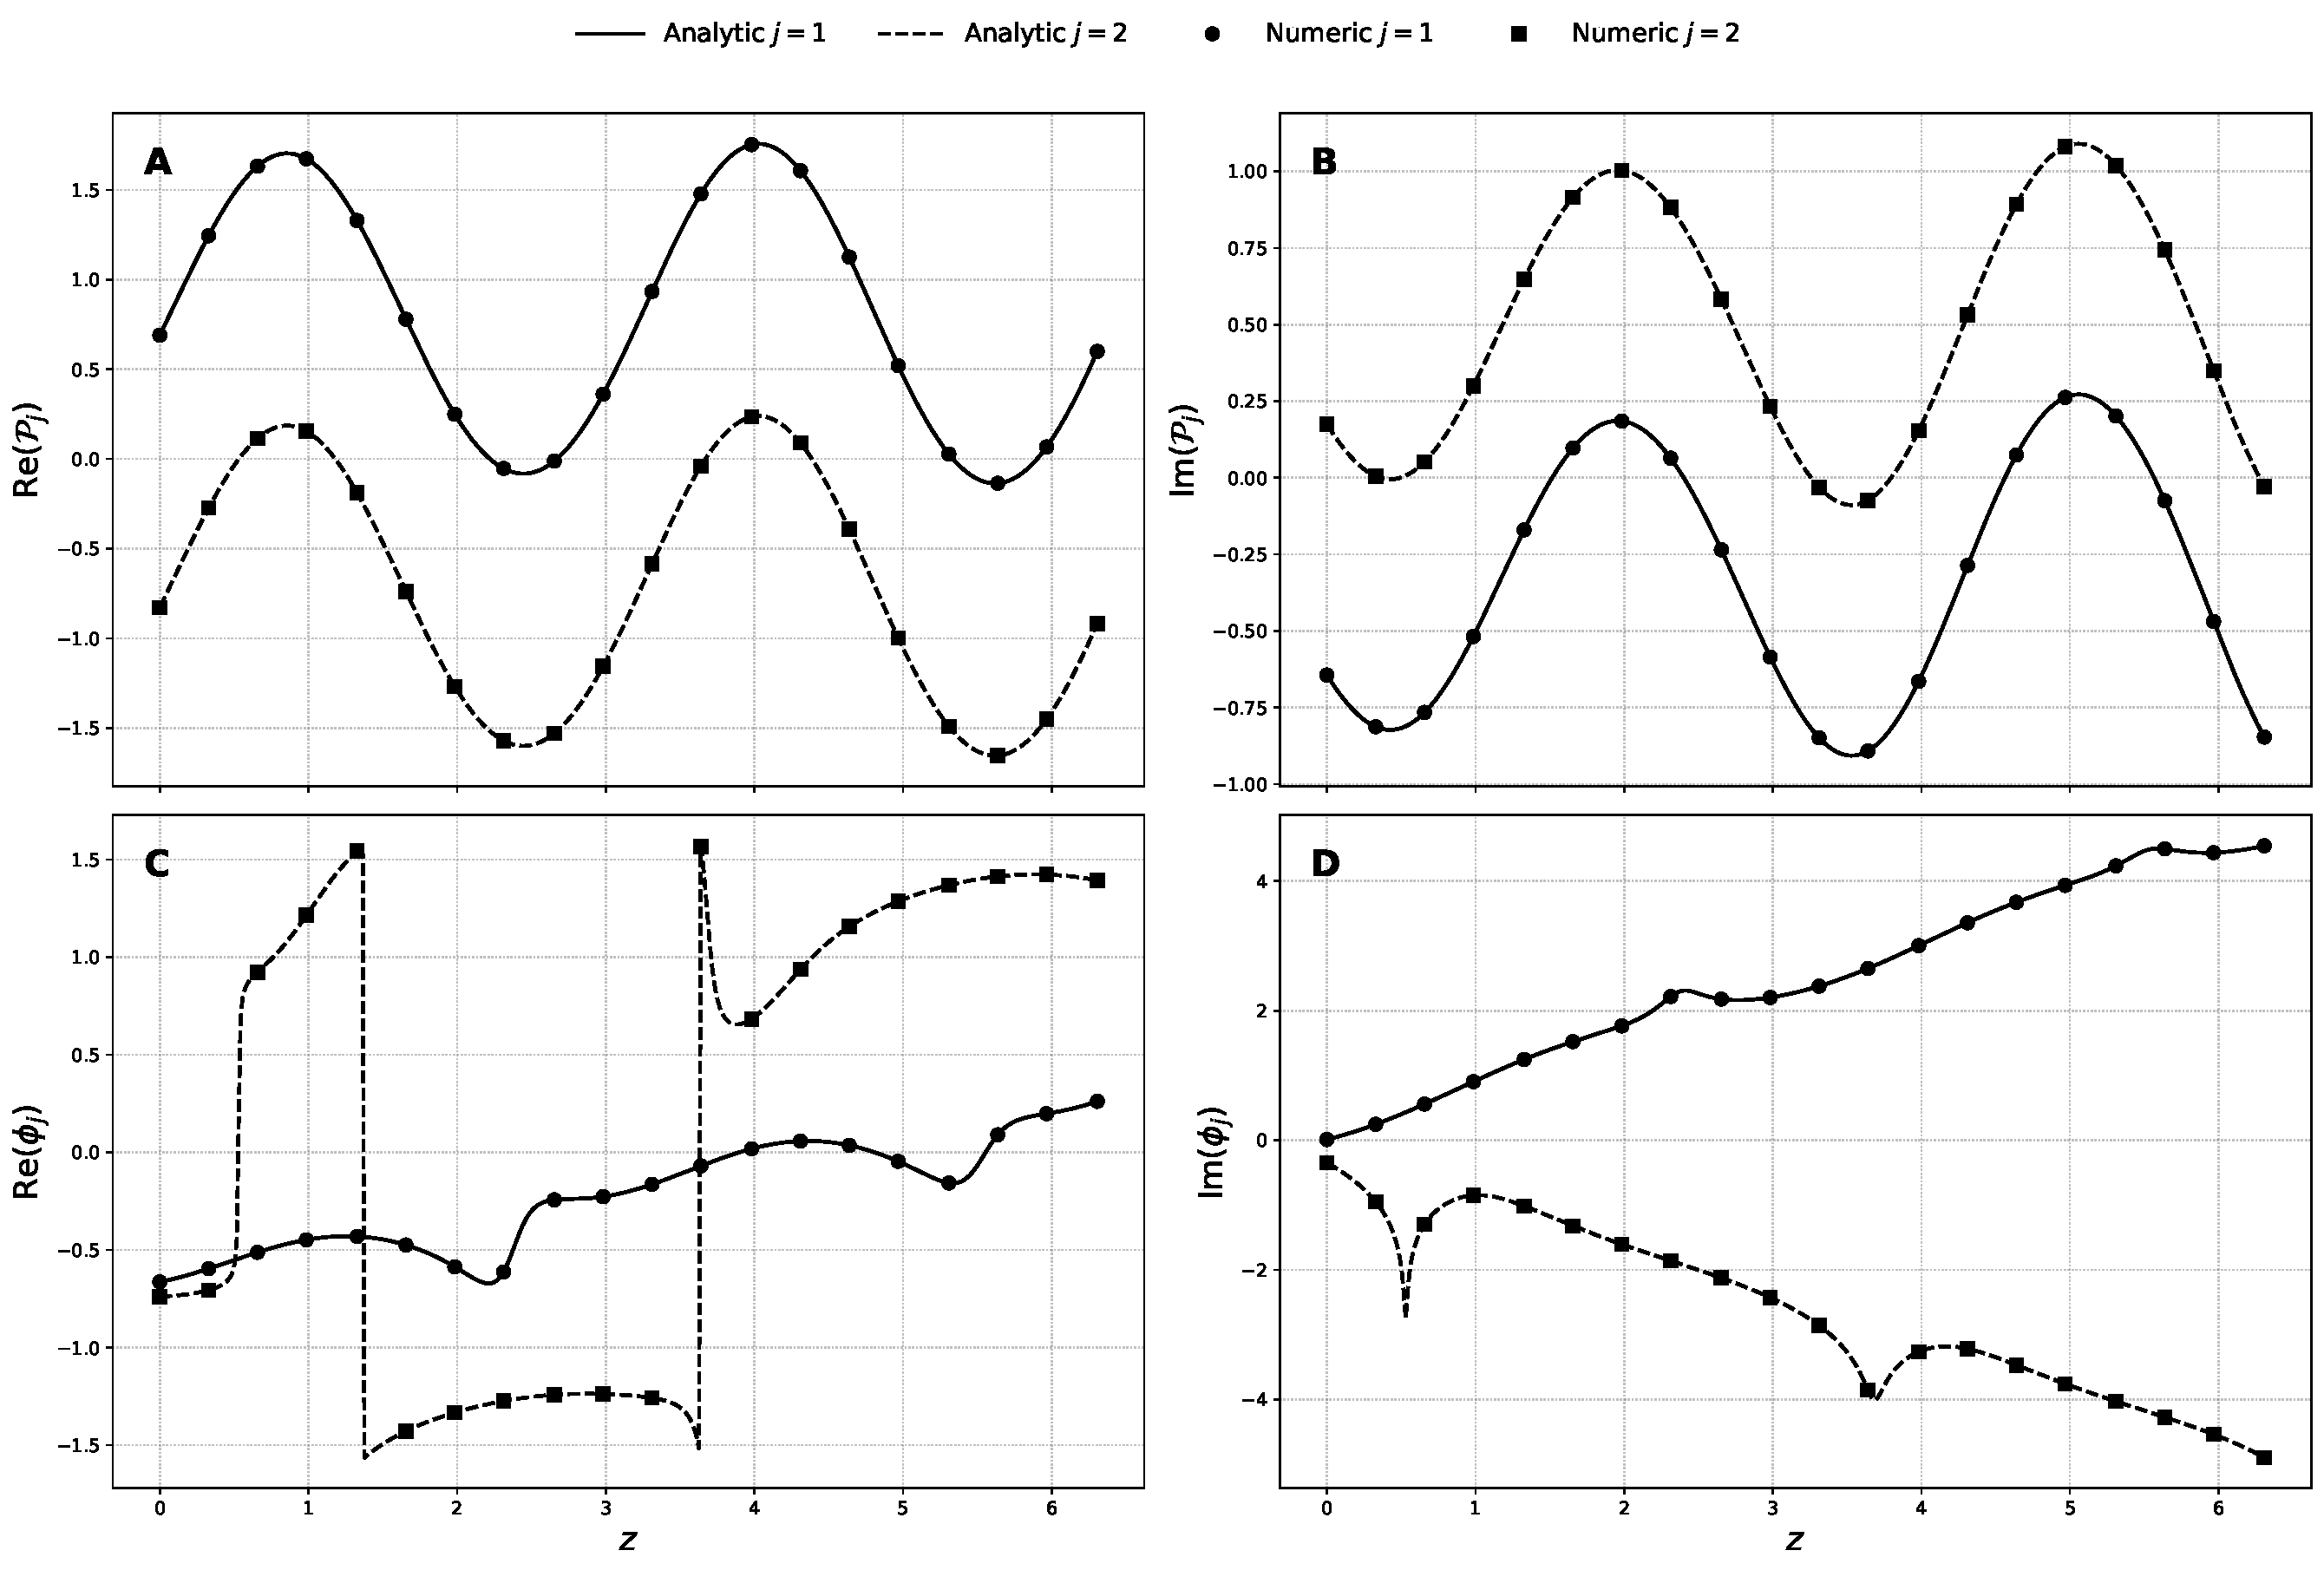
\includegraphics[width=1.0\textwidth]{plots/case1_plot_1.pdf}
\caption{\textbf{A} real and \textbf{B} imaginary parts of the complex mode power $A_j^2$, and \textbf{C} real and \textbf{D} imaginary parts of the complex phase variable $\phi_j$, using the analytic solutions in \eqref{eq:u-v-quartic} (lines) compared against numerical integration of the original general coherent coupler system in \eqref{eq:uv-system} (symbols).}
\label{fig:case1-plot1}
\end{figure}

\begin{figure}[H]
\centering
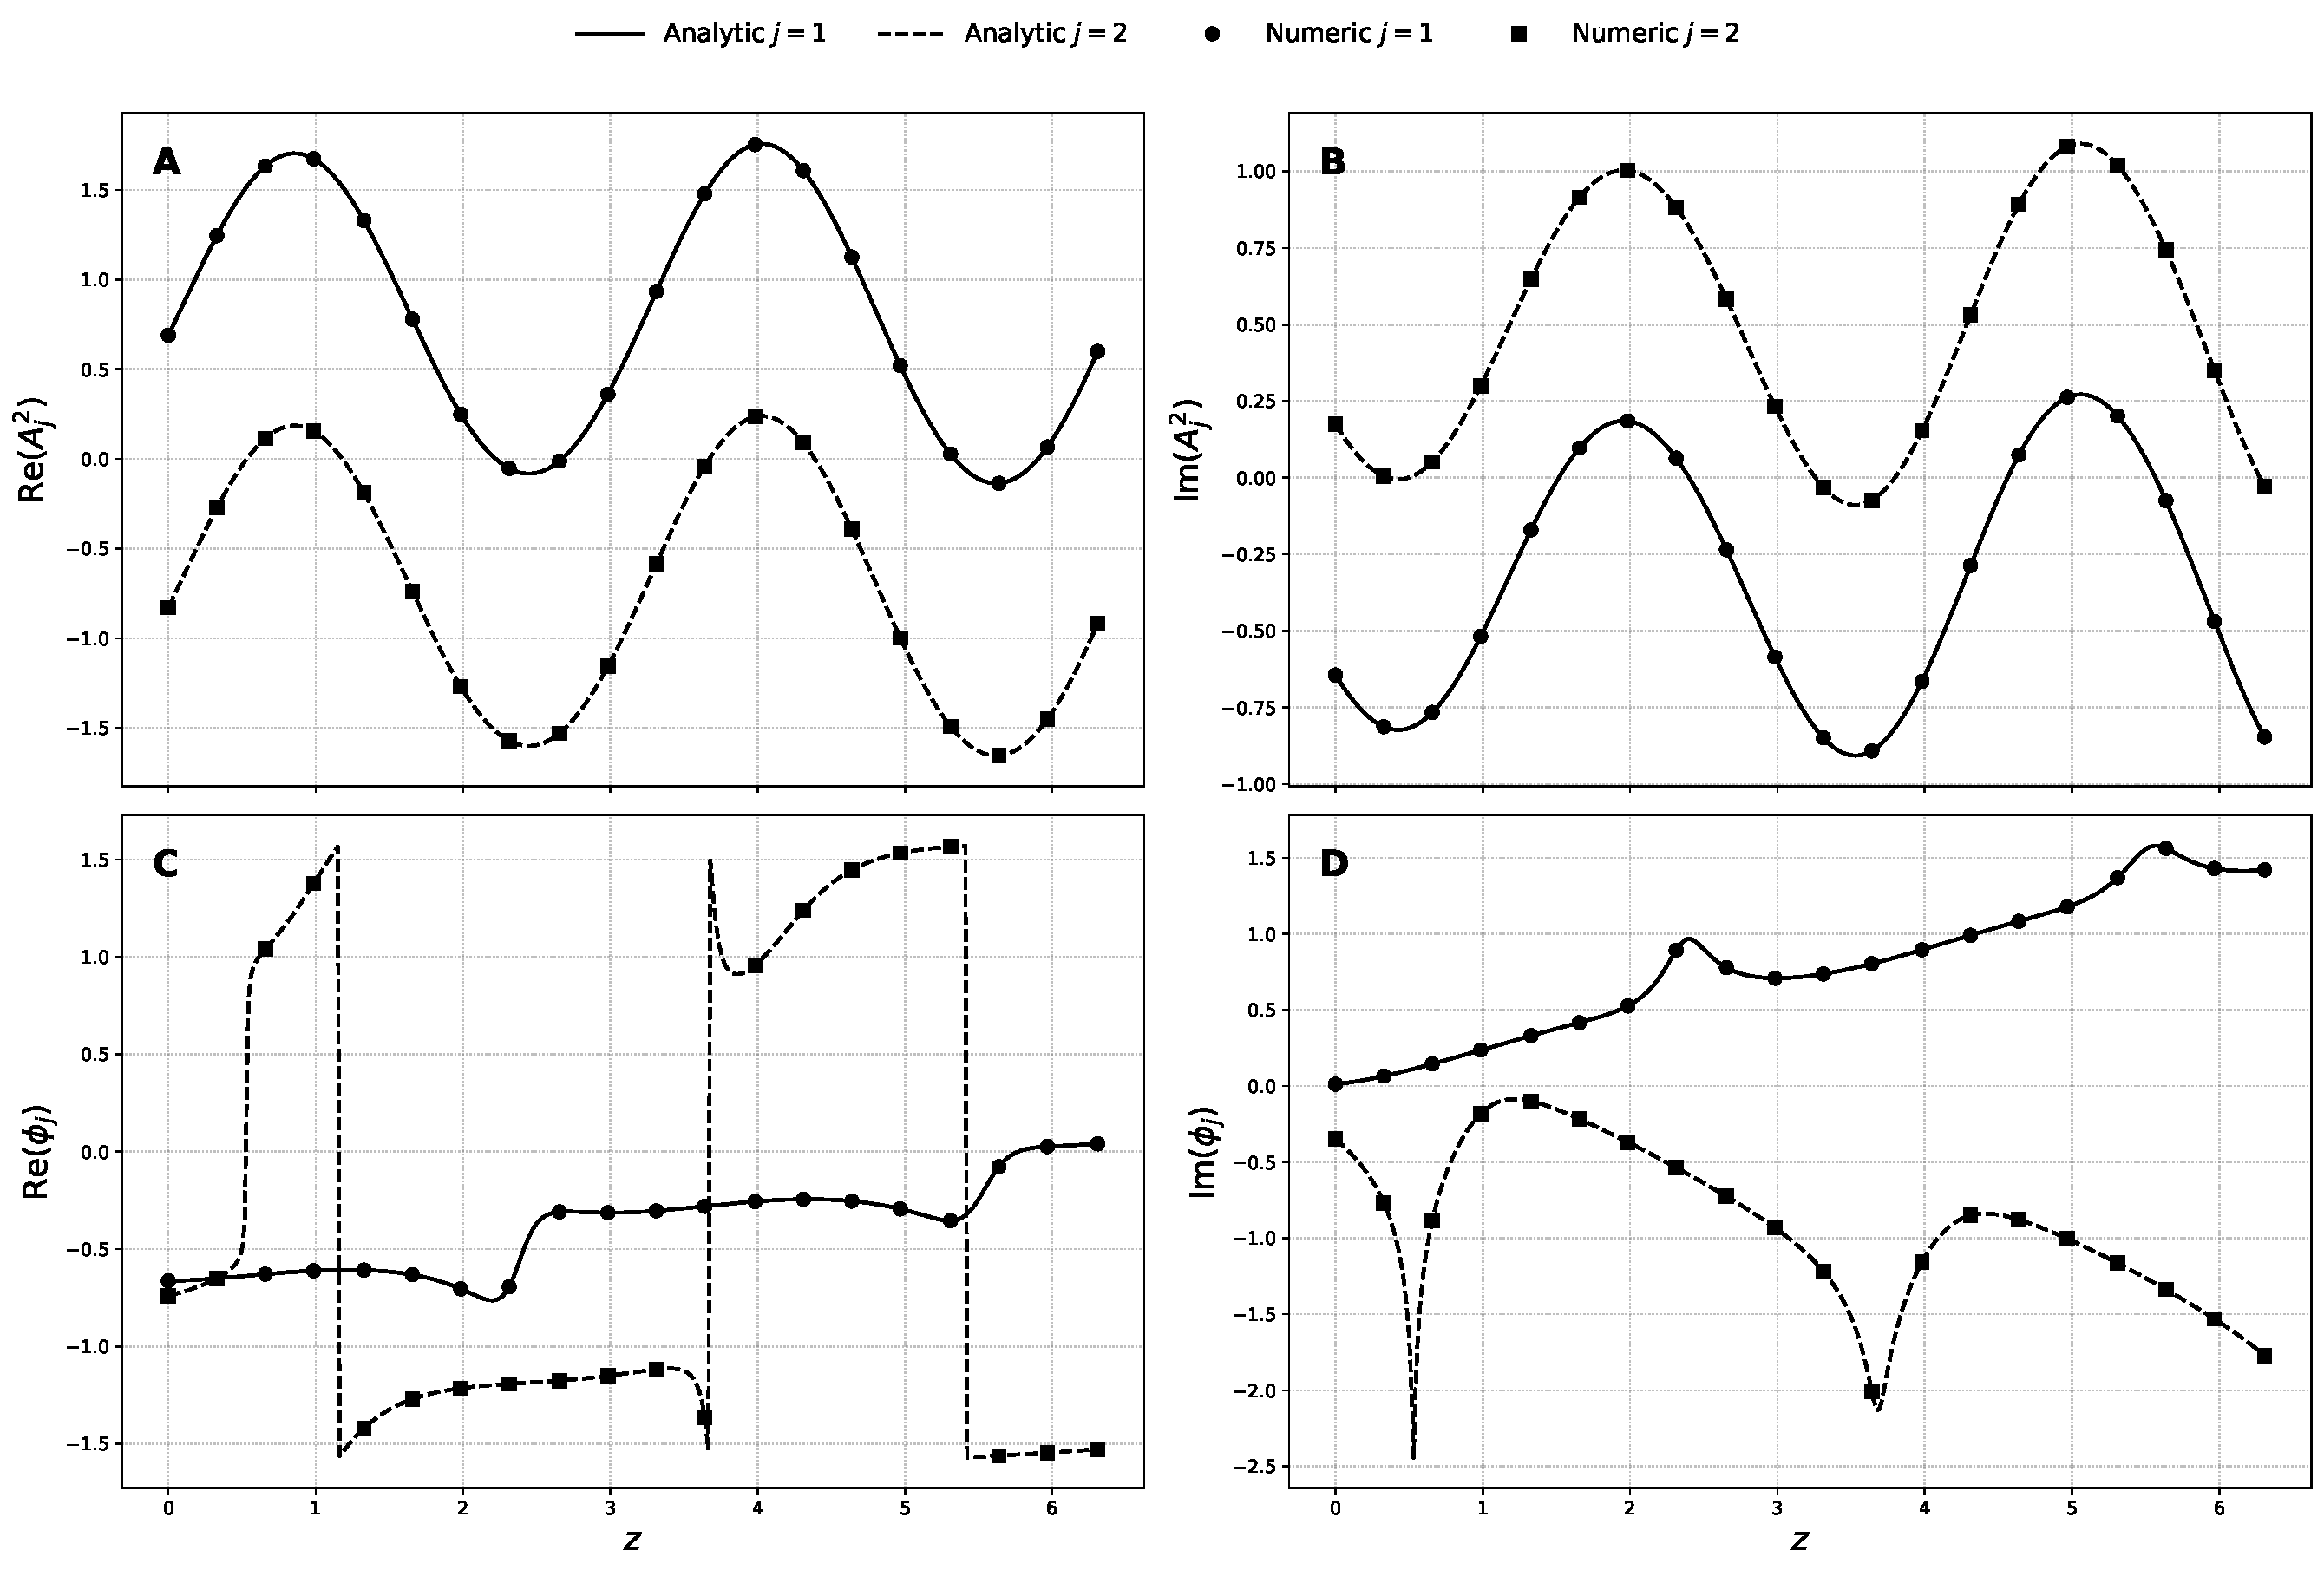
\includegraphics[width=1.0\textwidth]{plots/case2_plot_1.pdf}
\caption{\textbf{A} real and \textbf{B} imaginary parts of the complex mode power $A_j^2$, and \textbf{C} real and \textbf{D} imaginary parts of the complex phase variable $\phi_j$, using the gauge transformed analytic solutions in \eqref{eq:uhat-vhat-gauge-sols} (lines) compared against numerical integration of the gauge transformed general coherent coupler system in \eqref{eq:uv-hat-system} (symbols).}
\label{fig:case2-plot1}
\end{figure}

\begin{figure}[H]
\centering
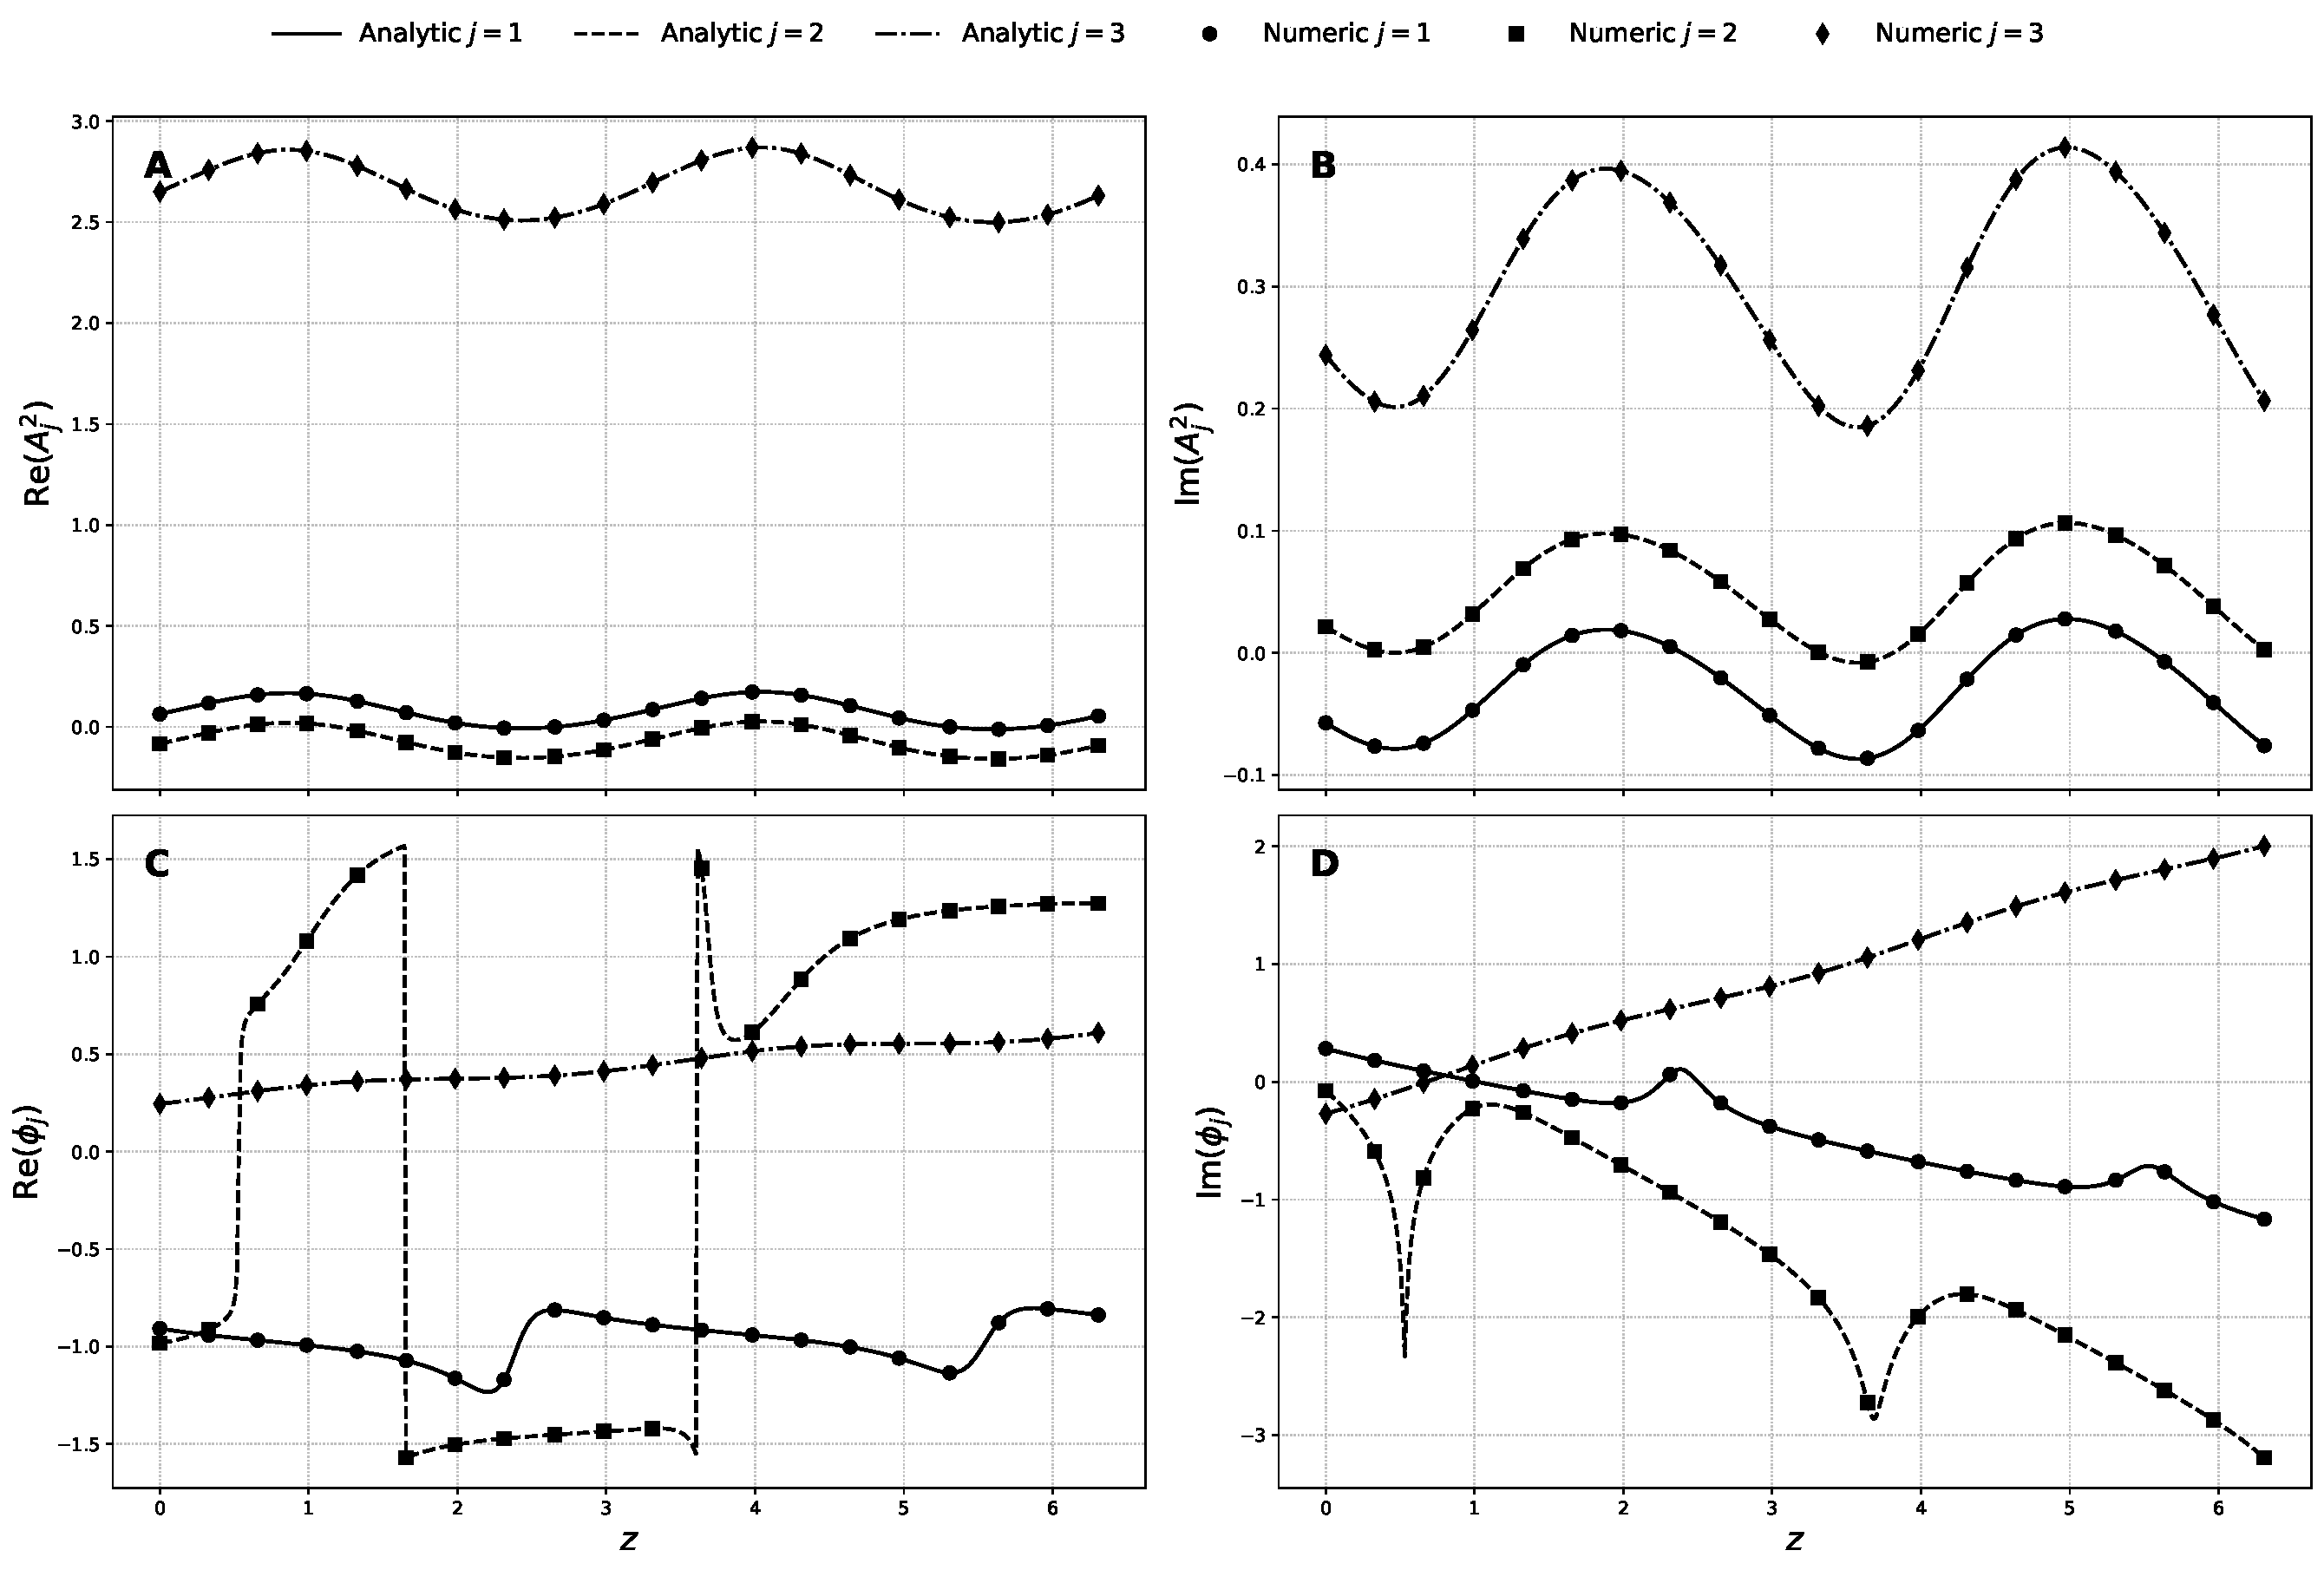
\includegraphics[width=1.0\textwidth]{plots/case3_plot_1.pdf}
\caption{\textbf{A} real and \textbf{B} imaginary parts of the complex mode power $A_j^2$, and \textbf{C} real and \textbf{D} imaginary parts of the complex phase variable $\phi_j$, using the analytic solutions in \eqref{eq:-ubar-vbar-sols-dfwm} (lines) compared against numerical integration of the three-mode degenerate FWM system in \eqref{eq:ubar-vbar-degfwm-system} (symbols).}
\label{fig:case3-plot1}
\end{figure}

\section{Conclusion}

We have presented complete analytic solutions for the generalised coherent coupler in nonlinear optics without the symmetric-parameter assumptions used in many treatments.
The solutions, expressed in terms of Weierstrass elliptic functions, provide the full complex field envelopes for all modes under generic initial conditions, including cross-phase modulation and phase mismatch effects.
These solutions complement previous work in the literature by providing a unified treatment of the complex envelopes themselves rather than treating amplitudes and phases separately.

Guided by the structure of these solutions, we explored coordinate transformations that reveal a projection from degenerate FWM to the generalised coherent coupler. 
The solutions in the degenerate FWM system are single-valued meromorphic Kronecker theta functions, connecting this work to a broader class of integrable nonlinear optical systems.

The connection between the Hamiltonian formulation and the Frobenius-Stickelberger determinant, established in Appendix~\ref{app:fs-det-ham-proof}, provides deeper insight into why these conservation laws hold and links four-wave mixing to classical elliptic function theory.
This mathematical framework may prove valuable for analysing related parametric processes and could extend to higher-order mixing or multimode interactions.

The methods developed here may be applicable to related nonlinear systems.
In particular, the approach may be transferable to the analysis of mode coupling in multimode nonlinear fibre optics (see, e.g., Chapter 4 in \cite{heskethNonlinearEffectsMultimode2014}), where similar coupled-mode structures arise.

The practical utility of these solutions has been demonstrated through numerical evaluation using open-source Python libraries, confirming both their validity and computational accessibility.
These analytic solutions may provide new insights for the design and optimisation of wavelength converters, parametric amplifiers, and quantum light sources by enabling exact analysis where approximations previously proved inadequate.


\section*{Acknowledgements}
The author thanks Maria Dimou for a careful read of the manuscript.

\section*{Code Availability}
The code used in this paper is available at \cite{heskethHeskethGDFwmpaper2026} and includes Python Jupyter notebooks with symbolic derivations using \emph{SymPy} \cite{meurerSymPySymbolicComputing2017} as well as the code for numerical validation used in Section~\ref{sec:num-val}.

\appendix


% ---------- APPENDIX ------------
% --------------------------------

\section{Parameter definitions in the original coordinates}
\label{app:param-def-appendix}

This appendix provides explicit formulae for the parameters $b_l$, $c_l$, and $d_l$ that appear in the quartic polynomial \eqref{eq:drho-sqrd-3} and related expressions throughout Section~\ref{sec:mode-power}.
These parameters are expressed in terms of the system parameters $a_j$, $a_{j,k}$ and the conserved constants $\gamma_j$.

\begin{align}
N &= 2,\\
{b}_{0} &= {a}_{0} + \sum_{j=1}^{N} {a}_{j} {\gamma}_{j} + \frac{1}{2}\sum\limits_{j,k=1}^{N} {a}_{j,k} {\gamma}_{j} {\gamma}_{k}, \notag \\
{b}_{1} &= - \sum_{j=1}^{N} {a}_{j} - \frac{1}{2}\sum\limits_{j,k=1}^{N} \left({\gamma}_{j} + {\gamma}_{k}\right) {a}_{j,k}, \notag \\
{b}_{2} &= \frac{1}{N}\sum\limits_{j,k=1}^{N} {a}_{j,k}, \notag \\
{c}_{0} &= \prod_{j=1}^{N} {\gamma}_{j}, \notag \\
{c}_{1} &= 0, \notag \\
{c}_{2} &= 1, \notag \\
{d}_{0} &= {b}_{0}^{2} - 4 {c}_{0}, \notag \\
{d}_{1} &= 2 {b}_{0} {b}_{1}, \notag \\
{d}_{2} &= 2 {b}_{0} {b}_{2} + {b}_{1}^{2} - 4, \notag \\
{d}_{3} &= 2 {b}_{1} {b}_{2}, \notag \\
{d}_{4} &= {b}_{2}^{2}
\end{align}

% ---------- APPENDIX ------------
% --------------------------------

\section{Initial condition relations}
\label{app:init-conds}

This appendix gives the relationships between initial conditions for the physical system and the constants $\gamma_j$ and $\rho(0)$ used throughout the analysis.
These relations enable determination of the constants from specified initial values of $u_j(0)$ and $v_j(0)$.

\begin{align}
N &= 2, \notag \\
\rho{\left(0 \right)} &= - \frac{1}{N}\sum_{j=1}^{N} u_j{\left(0 \right)} v_j{\left(0 \right)}, \notag \\
\left. \frac{d}{d z} \rho{\left(z \right)} \right|_{\substack{ z=0 }} &= \prod_{j=1}^{N} u_j(0) - \prod_{j=1}^{N} v_j(0), \notag \\
{\gamma}_{j} &= u_j{\left(0\right)} v_j{\left(0 \right)} + \rho{\left(0 \right)}
\end{align}


% ---------- APPENDIX ------------
% --------------------------------

\section{The Frobenius-Stickelberger determinant}
\label{app:fs-det-ham-proof}

The Frobenius-Stickelberger (FS) determinant formula is an elliptic function identity relating products of $\sigma$ functions to determinants of derivatives of $\wp$ \cite{whittakerCourseModernAnalysis2021, frobeniusZurTheorieElliptischen1877}.
In this appendix we demonstrate that the conservation of the Hamiltonian can be viewed as a manifestation of this classical identity, providing a deeper structural understanding of why the Hamiltonian is conserved in the coherent coupler.

Our starting point is equation \eqref{eq:fs-det-start}, which relates the wave mixing product to the phase modulation terms via the Hamiltonian.
We show that this equation can be transformed into the FS determinant formula by treating the left-hand side (the product of modes) and right-hand side (the polynomial in $\rho$) separately, each ultimately expressed in terms of Weierstrass functions.

We are interested in the $4\times4$ case of FS in the form:
\begin{align}
\label{eq:fs-det-m}
\frac{C\,\sigma{\left(z + {\nu}_{1}\right)} \sigma{\left(z + {\nu}_{2}\right)} \sigma{\left(z + {\nu}_{3}\right)} \sigma{\left(z - {\nu}_{1} - {\nu}_{2} - {\nu}_{3}\right)}}{\sigma^{4}{\left(z\right)}} & = \det M
\end{align}
where:
\begin{align}
C = &\frac{12  \sigma{\left({\nu}_{1} - {\nu}_{2}\right)} \sigma{\left({\nu}_{1} - {\nu}_{3}\right)} \sigma{\left({\nu}_{2} - {\nu}_{3}\right)} }{\sigma{\left({\nu}_{1}\right)} \sigma^{4}{\left({\nu}_{2}\right)} \sigma^{4}{\left({\nu}_{3}\right)}} \\[6pt]
\det M = &
\begin{vmatrix}
1 & \wp(z) & \frac{\partial \wp(z)}{\partial z} & \frac{\partial^2 \wp(z)}{\partial z^2} \\
1 & \wp(\nu_1) & -\frac{\partial \wp(\nu_1)}{\partial \nu_1} & \frac{\partial^2 \wp(\nu_1)}{\partial \nu_1^2} \\
1 & \wp(\nu_2) & -\frac{\partial \wp(\nu_2)}{\partial \nu_2} & \frac{\partial^2 \wp(\nu_2)}{\partial \nu_2^2} \\
1 & \wp(\nu_3) & -\frac{\partial \wp(\nu_3)}{\partial \nu_3} & \frac{\partial^2 \wp(\nu_3)}{\partial \nu_3^2} \\
\end{vmatrix}  \notag \\[6pt]
= & - 6 \left(\wp{\left({\nu}_{1}\right)} - \wp{\left(z\right)}\right) \left(\wp{\left({\nu}_{2}\right)} - \wp{\left(z\right)}\right) \left(\wp{\left({\nu}_{1}\right)} - \wp{\left({\nu}_{2}\right)}\right) \wp'{\left({\nu}_{3}\right)} \notag \\
& + 6 \left(\wp{\left({\nu}_{1}\right)} - \wp{\left(z\right)}\right) \left(\wp{\left({\nu}_{3}\right)} - \wp{\left(z\right)}\right) \left(\wp{\left({\nu}_{1}\right)} - \wp{\left({\nu}_{3}\right)}\right) \wp'{\left({\nu}_{2}\right)}  \notag \\
& - 6 \left(\wp{\left({\nu}_{2}\right)} - \wp{\left(z\right)}\right) \left(\wp{\left({\nu}_{3}\right)} - \wp{\left(z\right)}\right) \left(\wp{\left({\nu}_{2}\right)} - \wp{\left({\nu}_{3}\right)}\right) \wp'{\left({\nu}_{1}\right)}  \notag \\
& - 6 \left(\wp{\left({\nu}_{1}\right)} - \wp{\left({\nu}_{2}\right)}\right) \left(\wp{\left({\nu}_{1}\right)} - \wp{\left({\nu}_{3}\right)}\right) \left(\wp{\left({\nu}_{2}\right)} - \wp{\left({\nu}_{3}\right)}\right) \wp'{\left(z\right)}
\end{align}

The starting point for us is the following relation established via \eqref{eq:ham-uv}, \eqref{eq:duv_j}, and \eqref{eq:Q-uv}, where any choice of $j$ may be used in the modal-power derivative:
\begin{align}
2 \prod_{k=1}^{2} u_k &= {a}_{0} + \sum_{k=1}^{2} {a}_{k} u_k v_k  + \frac{1}{2}\sum\limits_{k,l=1}^{2} {a}_{k,l} u_k v_k u_l v_l - \frac{\partial}{\partial z}(u_j v_j) \notag \\
&=\rho' + \sum_{l=0}^{2}b_l\,\rho\left(z\right)^l. \label{eq:fs-det-start}
\end{align}
We now transform \eqref{eq:fs-det-start} into \eqref{eq:fs-det-m}.

\subsection{The left-hand side}
From \eqref{eq:uv-wp}, the right-hand side of \eqref{eq:fs-det-start} is a doubly periodic elliptic function, and therefore so is the left-hand side. Thus for integers $m,n$ and half-periods $\omega_1, \omega_3$ we must have:
\begin{align}
\prod_{j=1}^{2} \frac{u_j{\left(z\right)}}{u_j{\left(2 m {\omega}_{3} + 2 n {\omega}_{1} + z\right)}} & = 1. \label{eq:u-prod-is-one}
\end{align}
We substitute our solution \eqref{eq:u-v-quartic} into \eqref{eq:u-prod-is-one}, take advantage of \eqref{eq:r1j-sum} to simplify, and use the quasi-periodicity of $\sigma$:
\begin{align}
\sigma{\left(2 m {\omega}_{3} + 2 n {\omega}_{1} + z\right)} = \left(-1\right)^{m n + m + n} \sigma{\left(z\right)} e^{\left(2 m {\omega}_{3} + 2 n {\omega}_{1} + 2 z\right) \zeta{\left(m {\omega}_{3} + n {\omega}_{1}\right)}} \label{eq:quasi-sigma}
\end{align}
to reduce the product in \eqref{eq:u-prod-is-one} to an exponential which, as it is equal to one, must have argument $2\pi i \mathrm{N}(n,m)$, with $\mathrm{N}(n,m)$ an integer that varies with $n,m$.
For the lattice displacement determined by $2 z_1+\nu_1+\nu_2$, this gives:
\begin{align}
2 i \pi \mathrm{N}{\left(n,m \right)} &= - 2 \left(2 z_{1} + \sum_{j=1}^{2} {\nu}_{j}\right) \zeta{\left(m {\omega}_{3} + n {\omega}_{1},g_{2},g_{3} \right)} - \left(2 m {\omega}_{3} + 2 n {\omega}_{1}\right) \sum_{j=1}^{2} {r}_{0,j}, \label{eq:exp-arg-is-one} \\ 
2 z_{1} + \sum_{j=1}^{2} {\nu}_{j} &= 2 m {\omega}_{3} + 2 n {\omega}_{1} = 0 \pmod{\text{lattice}}, \label{eq:nuj-sum-zero}  \\
\sum_{j=1}^{2} {r}_{0,j} &= - 2 \zeta{\left(m {\omega}_{3} + n {\omega}_{1},g_{2},g_{3} \right)}. \label{eq:roj-is-zeta} 
\end{align}
where $\nu_j=\mu_j-z_0$, and where the integers $m,n$ in \eqref{eq:nuj-sum-zero} specify the relevant lattice point rather than arbitrary independent periods.
In moving from \eqref{eq:exp-arg-is-one} to \eqref{eq:nuj-sum-zero} and \eqref{eq:roj-is-zeta} we made use of the identity $\zeta{\left({\omega}_{3}\right)} {\omega}_{1} - \zeta{\left({\omega}_{1}\right)} {\omega}_{3} = i \pi /2$. 
Ultimately, equations \eqref{eq:quasi-sigma}, \eqref{eq:nuj-sum-zero} and \eqref{eq:roj-is-zeta} allow us to make the following substitution (or the equivalent at $z\rightarrow z - z_0$) in the left-hand side of \eqref{eq:fs-det-start}:
\begin{align}
\frac{\sigma{\left(z + z_1 \right)}}{\sigma{\left(z_1 \right)}}\,\exp{\left(z \sum\limits_{j=1}^{2} {r}_{0,j}\right)} = - \frac{\sigma{\left(z - z_1 - {\nu}_{1} - {\nu}_{2}\right)}}{\sigma{\left(z_1 + {\nu}_{1} + {\nu}_{2}\right)}}.
\end{align}

\subsection{The right-hand side}
The following polynomial interpolation formula holds for any quadratic polynomial:
\begin{align}
\sum_{l=0}^{2}b_l\,\rho\left(z\right)^l =\, &\frac{{\gamma}_{1} - \rho{\left(z \right)} }{{\gamma}_{1} - {\gamma}_{2}} \sum\limits_{l=0}^{2}b_l\,\gamma_1^l + \notag \\
&\frac{{\gamma}_{2} - \rho{\left(z \right)} }{{\gamma}_{2} - {\gamma}_{1}} \sum\limits_{l=0}^{2}b_l\,\gamma_2^l + \notag \\
&\left({\gamma}_{1} - \rho{\left(z \right)}\right) \left({\gamma}_{2} - \rho{\left(z \right)}\right) b_2 \label{eq:poly-interp}
\end{align}
where, in our case, $\gamma_j=\rho(\mu_j)$ and the sum over $b_l \gamma_j^l$ can be written using \eqref{eq:drho-sqrd-2} as:
\begin{align}
\sum\limits_{l=0}^{2}b_l\,\gamma_j^l = \rho'\left(\mu_j\right).
\end{align}
We can then use \eqref{eq:uv-wp} to express $\rho$ in terms of $\wp$ so that all variables in \eqref{eq:poly-interp} can be written in terms of $\wp$ and $\wp'$. 
We then divide both sides of \eqref{eq:fs-det-start} by:
\begin{align}
\frac{\wp'{\left(z_{1}\right)}}{b_2 \left(\wp{\left(z_{1}\right)} - \wp{\left(z - z_{0}\right)}\right)^2 }
\end{align}
and observe that it takes the equivalent form to \eqref{eq:fs-det-m} up to constant factors that may look different but can be shown to be identical by evaluating at $z\rightarrow z + z_0$, multiplying by $\sigma(z)^4$, and taking $z\rightarrow 0$.

This completes the demonstration that the Hamiltonian conservation law \eqref{eq:fs-det-start} is equivalent to the Frobenius-Stickelberger determinant formula.
This connection reveals that the conserved Hamiltonian of the coherent coupler is not merely a convenient construct but rather a manifestation of deep structural properties of elliptic functions.


\printbibliography

\end{document}
